%# -*- coding: utf-8-unix -*-
%%==================================================
%% thesis.tex
%%==================================================

% 双面打印
\documentclass[master, fontset=adobe, openright, twoside]{sjtuthesis}
% \documentclass[bachelor, fontset=adobe, openany, oneside, submit]{sjtuthesis}
% \documentclass[master, fontset=adobe, review]{sjtuthesis}
% \documentclass[%
%   bachelor|master|doctor,	% 必选项
%   fontset=adobe|windows,  	% 只测试了adobe
%   oneside|twoside,		% 单面打印,双面打印(奇偶页交换页边距,默认)
%   openany|openright, 		% 可以在奇数或者偶数页开新章|只在奇数页开新章(默认)
%   zihao=-4|5,, 		% 正文字号:小四、五号(默认)
%   review,	 		% 盲审论文,隐去作者姓名、学号、导师姓名、致谢、发表论文和参与的项目
%   submit			% 定稿提交的论文,插入签名扫描版的原创性声明、授权声明 
% ]

% 逐个导入参考文献数据库
\addbibresource{bib/thesis.bib}
% \addbibresource{bib/chap2.bib}

\begin{document}

%% 无编号内容:中英文论文封面、授权页
%# -*- coding: utf-8-unix -*-
\title{面向ASR的结构化语言模型的研究}
\author{吴\quad{}越}
\advisor{俞凯教授}
% \coadvisor{某某教授}
\defenddate{2017年12月17日}
\school{上海交通大学}
\institute{电子信息与电器工程系}
\studentnumber{115033910029}
\major{计算机科学与技术}

\englishtitle{Research on structured language model for ASR}
\englishauthor{\textsc{Yue Wu}}
\englishadvisor{Prof. \textsc{Kai Yu}}
% \englishcoadvisor{Prof. \textsc{Uom Uom}}
\englishschool{Shanghai Jiao Tong University}
\englishinstitute{\textsc{Department of Computer Science and Engineering, School of Electronic Information and Electrical Engineering} \\ 
	 \textsc{Shanghai Jiao Tong University} \\  
	\textsc{Shanghai, P.R.China}}
\englishmajor{Computer Science and Technology}
\englishdate{Jan. 15th, 2017}


\maketitle

\makeenglishtitle

\makeatletter
\ifsjtu@submit\relax
	\includepdf{pdf/original.pdf}
	\cleardoublepage
	\includepdf{pdf/authorization.pdf}
	\cleardoublepage
\else
\ifsjtu@review\relax
% exclude the original claim and authorization
\else
	\makeDeclareOriginal
	\makeDeclareAuthorization
\fi
\fi
\makeatother


\frontmatter 	% 使用罗马数字对前言编号

%% 摘要
\pagestyle{main}
%# -*- coding: utf-8-unix -*-
%%==================================================
%% abstract.tex for SJTU Master Thesis
%%==================================================

\begin{abstract}

最近,长短时间变化神经网络语言模型(LSTM LM)因为它的记忆单元出色的对历史信息的记忆能力,得到了语言和语音学者广泛的关注。
对语言模型进行一系列的结构优化可以使其在自动语音识别任务中表现得更好。
本文首先针对语言模型的结构化特性进行学习率自适应的研究,
获得最好的调整方法,成功使得语言模型的不同结构能自动调整学习率,为后面研究工作打好基础。
接着,由于将辅助信息(如上下文特性)加入到LSTM LM中,能在语言模型的混淆度(PPL)中体现出比较大的语言模型的性能提升。
然而,在大量的词汇连续语音识别(LVCSR)任务中,辅助信息的不恰当的输入不会使单词错误率(WER)获得同样的增益。
为了解决这一问题,本文提出了一种多视角融合的LSTM语言模型结构。首先建立了一种在线单向lstm作为一种标记模型,可以生成词同步的辅助信息特征。
然后将标记模型的辅助特征与单词序列结合起来,训练多视角单向LSTM语言模型。研究并比较了不同的标记模型和语言模型的训练模式。
在英文数据集PTB、Fisher和中文短信S数据集上对新架构进行了评价,结果表明,新的模型结构不仅能够提升混淆度,也能减小语音识别任务中的词错误率和句子错误率。
除此之外,本文将教师-学生模型引入到语言模型中,
探究多种模型之间的教授方式,并最终能大幅度提升小语言模型的性能。


\keywords{\large 关键词: \quad 自动语音识别 \quad 语言模型 \quad 神经网络 \quad 多视角语言模型 \quad 学习率自适应 \quad 教师-学生模型}
\end{abstract}

\begin{englishabstract}
Recently long short-term memory language model (LSTM LM) has received tremendous interests from both language and speech communities, 
due to its superiorty on modelling long-term dependency. 
A series of structural optimizations to the language model can make it perform better in auto speech recognition tasks.
In this paper, we firstly concern learning rate adaption task aiming at the structural characteristics of the language model.
The best adjustment method is obtained, which enables the different structure of language model to automatically adjust the learning rate and lay a foundation for the research work in the future.
Later, because integrating auxiliary information, 
such as context feature, into the LSTM LM has shown improved performance in perplexity (PPL). 
However, improper feed of auxiliary information won't give consistent gain on word error rate (WER) in a large vocabulary continuous speech recognition (LVCSR) task. 
To solve this problem, a multi-view LSTM LM architecture combining a tagging model is proposed in this paper.
 Firstly an on-line unidirectional LSTM-RNN is built as a tagging model, which can generate word-synchronized auxiliary feature. 
Then the auxiliary feature from the tagging model is combined with the word sequence to train a multi-view unidirectional LSTM LM. 
Different training modes for the tagging model and language model are explored and compared. The new architecture is evaluated on PTB, 
Fisher English and SMS Chinese data sets, and the results show that not only LM PPL promotion is observed, but also the improvements can be well transferred to WER reduction in ASR-rescore task.
In addition, this paper introduces the teacher - student model into the language model.
Explore the way of teaching among various models and ultimately improve the performance of small language models.
\englishkeywords{\large ASR, language model, neural network, multi-view, learning rate adaptation, teacher-student model}
\end{englishabstract}



%% 目录、插图目录、表格目录
\tableofcontents
\listoffigures
\addcontentsline{toc}{chapter}{\listfigurename} %将插图目录加入全文目录
\listoftables
\addcontentsline{toc}{chapter}{\listtablename}  %将表格目录加入全文目录
\listofalgorithms
\addcontentsline{toc}{chapter}{算法索引}        %将算法目录加入全文目录

\include{tex/symbol} % 主要符号、缩略词对照表

\mainmatter	% 使用阿拉伯数字对正文编号

%% 正文内容
\pagestyle{main}
%# -*- coding: utf-8-unix -*-
%%==================================================
%% chapter01.tex for SJTU Master Thesis
%%==================================================

%\bibliographystyle{sjtu2}%[此处用于每章都生产参考文献]

\chapter{绪论}
\label{chap:intro}
\section{语言模型及其研究背景}
随着计算机运行速度的提升和机器学习领域的发展,机器学习已经成为当今大的研究趋势。
智能语音可以让计算机听懂甚至理解人类的语言,因此成为了智能交互中很重要的一部分,语言模型的作用功不可没。
同时,大规模语料库的出现和现代计算机计算能力的提升,为自然语言统计处理方法的实现提供了可能,统计方法的成功使用推动了语言模型的发展。
语言模型作为衡量一句话的流畅及合理程度的模型,语言模型在语音识别和自然语言处理任务中都得到了广泛的应用。
在自然语言处理任务中,语言模型不仅可以用来衡量语句的符合语言规律及通顺程度,更可以和众多别的自然语言处理任务相辅相成,相互促进。
在语音识别任务中,语言模型和声学模型合作完成,通过解码过程将音频信息转化为最为合理的文字。
本论文着重介绍语言模型在语音识别任务中的研究和优化。



自古以来,语音都是人类最重要的交流方式之一。
自电话发明以来,学者们致力于机器的语音的研究工作。
19世纪晚期,在语音工作的种种问题中,自动语音识别(Automatic Speech Recognition,ASR)成为最具挑战性和吸引力的任务之一,它是通过先记录语音波形并通过一系列算法自动转换为文本。
然而,对ASR的研究在20世纪初却进展缓慢,甚至1969年,贝尔实验室的约翰·皮尔斯还曾声称自动语音识别在几十年内不会成为现实。


不过,在十九世纪70年代,语音识别领域有了巨大的突破。
各类方法在语音识别领域崭露头角,其中就包括语言模型。
在接下来的几十年里,随着机器学习方法的提出,和深度学习的证实与应用,神经网络被用于语音识别领域。
基于神经网络的各种语言模型训练方法也逐步进入研究者的视角。
在此基础上,各种结构化神经网络的语言模型相关研究再一次推动了语言模型的性能和应用空间。


语音识别系统的目的是能通过给定的语言波形而产生一个单词序列(或者可能是适用于普通话之类语言的汉字序列)。


ASR系统的基本结构如图\ref{fig:asr}所示\cite{mohamed2012acoustic}。



\begin{figure}[!htbp]
  \centering
  \begin{minipage}[b]{0.6\textwidth}
    \captionstyle{\centering}
    \centering
    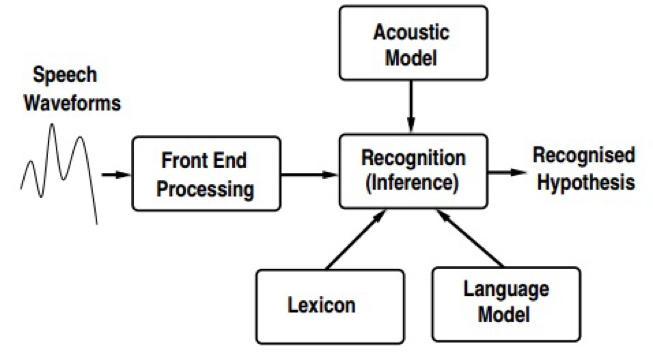
\includegraphics[width=12cm]{intro/ASR.png}
    \bicaption[fig:asr]{自动语音识别系统}{ASR structure}{Fig}{自动语音识别系统的结构}
  \end{minipage}     
\end{figure}

语音识别的第一阶段是压缩语音信号(逐帧)为声学特征向量的流, 称为观测值。

提取的观测向量被设计成包含足够的信息以及足够紧凑来执行有效的语音识别。
这一过程被称为前端处理或特征提取。
/
从观测特征向量说开来,ASR系统可分为三个主要部分:词汇,语言模型和声学模型。

词汇或者称为词典,用于映射出在声学模型中的子字单元到词汇与语言模型中的实际单词。
语言模型代表了已说出句子的当地句法和语义信息。
它对每个单词序列都分配了个可能性。
声学模型,通常是语音研究者们最感兴趣的,映射了语音观测值到子字单元。
 GMM-HMM框架一直是ASR框架的最先进技术,直到最近深度神经网络(DNN)被引入到ASR系统中。
计划中的深度神经网络HMM(DNN-HMM)相比于最先进的GMM-HMM来说在两种任务上都取得了显著进步,音素识别\cite{mohamed2012acoustic}和大词汇连续语音识别(LVCSR)\cite{dahl2012context}任务。
它使用一个深度神经网络(DNN)来计算聚类后状态并将其转换为可用于HMM的状态和条件似然概率。


深度神经网络(DNN)比起浅层的神经网络有更强大的模拟/建模能力。
但是, 它也更有可能因为正常初始化策略和反向传播(BP)优化而陷入局部的最优。
RBM(受限玻耳兹曼机)的预训练\cite{mohamed2012acoustic}或区别预训练\cite{bengio2007greedy}被提出来用作初始化权重矩阵到一个更好的起点,这使BP微调过程更容易,而且收敛更快速。
最近,文献\cite{mohamed2010investigation}\cite{vesely2013sequence}介绍了更先进的训练标准,它们已被应用于得到更精确的模型。
除了混合框架,DNN也可以用于获得更完善的瓶颈特征\cite{yu2011improved},以训练GMM-HMM系统并已经实现了与DNN相匹配的性能。


随着自动化语音识别的不断优化和发展,在识别中扮演重要角色的语言模型的研究同样得到迅速发展。
从传统的统计学语言模型N-gram到神经网络语言模型,从普通的深度神经网络语言模型到有历史记忆功能的循环神经网络,再到更优秀但是更复杂的长短时间变化神经网络,甚至是各种对模型结构上的优化,一步步使语言模型研究更加深入,从而大幅度提升语言模型的性能。



\section{语言模型的相关研究}
在20世纪90年代,最初的语言模型N-gram语言模型开始被提出。
N-gram语言模型原理简单,仅需要掌握简单的概率论基础知识和极大似然概率就能实现,而且速度很快,对于当时的计算机硬件条件来说适用性很高,很快就被广泛接受和应用开来。
这样一来,很多缺点和不足也就暴露出来,比如当训练数据不足的情况下很容易出现很多单词的预测概率为0,于是就有很多学者提出各种平滑算法来解决语料稀疏的问题。
比如基于二项后验分布的后退(back-off)平滑方法\cite{kawabata1996back},
基于普通计数的平滑方法\cite{moore2009improved}
和Kneser-Ney平滑\cite{pickhardt2014generalized}等。
其中Kneser-Ney平滑算法是目前比较标准的,而且是非常先进的平滑算法。

除了这些平滑算法,在N-gram的训练形式和语料的预处理方面专家们也是下足了功夫,
例如基于缓存的(Cache-based N-gram模型用缓存记录历史信息\cite{kuhn1990cache},
基于类别的(Class-based)N-gram模型将单词进行分类处理\cite{brown1992class}
以及基于话题的(Topic-based)N-gram模型在训练单词的时候为其配备话题附加信息以达到更好的训练等\cite{gildea1999topic}。

随着21世纪深度学习方法被证实可用,神经网络算法开始被用于自动语音识别和语言模型的学习当中。
开始的DNN算法由于无法记录较长的历史信息而不适用于语言模型,因为语言是具有前后文连贯性的。
接着随着RNN语言模型的提出,发现具有递归结构能够记录历史信息的循环神经网络(Recurent Neural Network,RNN)网络非常适用于语言模型。

RNN由于递归结构的存在使得语言的历史信息能够被记住,十分符合语言学的规律,使得语言模型的性能从统计模型N-gram有了很大的提升。
同时RNN模型的训练方式也从以前普通DNN的反向传播算法(BP)变化成了基于时间的反向传播算法(BPTT),这个算法将会在第二章进行详细介绍。
同样的,学者将优化N-gram语言模型的思想扩展到语言模型上,提出一系列优化RNN语言模型的算法。
例如Class based RNNLM被提出,它的思想同N-gram一样,对训练单词进行分类训练,能够有效的提高训练速度,并且对于丰富多彩的语言来说,那些出现概率偏小的词汇在预测中容易导致概率为0的问题得到了平滑。
优化深度神经网络(DNN)的各种训练算法同样适用于RNN语言模型的训练,从开始的一个词一个词的训练的随机梯度下降,到多个词同步训练的批量梯度下降,以及训练中加入块的机制,都大幅度提升了RNN模型的训练速度,同时也一定程度提升了语言模型的性能。
从语言模型训练速度的方向考虑,以前的语言模型不能同声学模型一样进行minibatch训练(nimibatch即是把训练数据分批输入到神经网络中进行学习),因为语言模型的识别往往和前后文以及历史信息关系密切,然而去年有学者提出可以换种方式考虑minibatch,同时读入很多句子,在不同的没有关联的句子中选取不同的单词进行minibatch输出,则不会影响学习相关性的情况下还能对速度有所提升。
另外多核并行学习,利用GPU和Intel函数库进行训练等方法逐渐被用于语言模型训练上。

然而RNN语言模型依然有一个普遍存在的问题——梯度消失。
即当语句过长时,距离现在较长的历史会随着一步步的递归使得历史影响消失,这种情况使得RNN虽然理论上能用到的历史信息是全部历史,但是真正产生作用的历史信息依然非常有限。
针对这个问题,
有人提出加入长短时间记忆(LSTM)的神经网络语言模型来学习那较长的句子。面对这些些有很长一段时间信息滞后并且滞后时间的长短未知的句子,它通过分割记忆块的形式控制误差的传递时机,训练得到语言模型的性能相比传统RNNLM具有一定提升。
好在无论是训练方法的提升(小批量随机梯度下降),还是计算方法的提升(多线程GPU并行)以及硬件计算能力的提升为训练具有相对于RNN来说几倍参数量的LSTM模型提供了可能性。

在上述技术基础上,针对基础语言模型进行的各种创新结构的研究也在紧锣密鼓的进行。
多视角(Multi-view)语言模型是将多种特征向量加入到语言模型中辅助训练更好的语言模型的结构,
比如加入前后文相关信息的RNN语言模型于近年被Mikolov提出,它在训练当前单词的时候加入前后文块,并为词性加入话题信息,结合话题模型一起进行训练,形成一个受话题制约的RNNLM,可以有效避免数据在不同类型的数据子集上训练话题模型导致的数据分裂。
多任务(Multi-task)学习同样受到了很大的关注,其主要思想是在训练语言模型时加入其它的任务混合训练,共用一定数量的隐藏层或参数矩阵,达到相互促进相互制约的作用。
联合学习(Joint train)作为多视角和多任务模型的结合,也是最复杂的一个。
不仅像多视角模型一样拥有多维视角特征,也像多任务学习一样多种不同任务共同学习以达到相互促进和泛化的作用。
往往多任务的输出会以各种经过尝试的较好方式作为额外视角加入到下个时间点的训练中。

上述提到的各种语言模型的结构化尝试也是本文的工作重点,额外的丰富的信息和合理的结构往往能使语言模型发挥更好的效果。







	
\section{本文的研究内容及贡献}

本课题主要研究面向ASR的结构化的语言模型,以提升语言模型的性能。
首先,本文调研所有现有的结构化语言模型的研究现状和它们的优缺点,以得到研究的突破点:大多数结构化模型的研究都仅仅提升了混淆度,而没有提升ASR重打分任务中的指标。
接着本文分析造成这个现象的原因:用不应该使用的含有后文信息的标注预测后文信息使得混淆度有巨大提升,但是这种提升是用到了作弊的后文信息,
而在语音识别的N-best重打分任务中,后文的信息不一定正确因此没有提升。
于是有了本文主要工作的研究动机:将单向信息抽象出来,进行Multi-view语言模型的训练,然后在N-best重打分实验中验证结果。


由于词层面的Multi-view必须使用此层面的信息。
为此我们优先调研有哪些词层面的信息,且哪些可以被用在我们的研究中。
最后得到了三种辅助特征:词性标注(POS),命名实体识别(NER),语法块标注(Chunking)。
其中有些可以直接通过现有工具获得标注,有些需要自己根据论文实现标注工具。

接下来是为结构化语言模型的研究作为辅助任务但仍十分钟要且有一定研究成果的任务:面向结构化语言模型的学习率自适应算法。
由于结构化的模型中,不同的结构会有不同的特性,且训练步调也不一定会一致,因此使用同一种学习旅会影响模型的学习效果。
我们在已有的$beta$稳定算子学习率自适应算法中,将其移植到LSTM语言模型中,保持了原有的效果,即使得模型对初始学习率不敏感,能自动调整模型在训练过程中的学习幅度,
从而使得无论是Multi-task还是Multi-view或者是Joint-train模型都能根据没一部分的特性有“个性”地进行学习。
在此基础上,对$beta$进行L2正则化优化,使其能一定程度上($1\%$)提升模型性能。
研究完整且颇有成效,最后我们也是将这个研究成果运用到本文的结构化语言模型的研究中去,最后使得研究更为系统和有说服力。

在本文的主要研究内容中,在上述辅助特征的选取和学习率自适应的基础上。
本文提出面向ASR的单向辅助信息的Multi-view语言模型,模型是一个整体,但是分成标注LSTM和Multi-viewLSTM语言模型两部分。
意在将不含后文信息更准确的辅助特征加入到语言模型中一起训练。
并且含有多种连接方式和多种训练方式。最后通过实验验证哪种方式更好,以及模型是否有效果。

实验部分首先选取合适的数据集,本文选取了中文和英文的数据集以试图得到更为普遍的结果。
在英文数据集上,也选取了较大的和较小的两种,其中中文和英文大数据集是能进行N-best重打分实验的。
除此之外还要将数据集预处理,分别通过对应的算法得到数据对应的词性、话题和场景等不同的信息,并进行标注得到新的数据集。
然后,以词为单位对带标记的数据进行解析,得到其词向量和对应信息的特征向量。
最后将这些向量一同作为标注模型进行训练。
模型的基线也是非常全面,除了统计学N-gram模型之外,还有普通的LSTM语言模型,和基础的Multi-view、Multi-task、Joint-train语言模型三种,来测试我们的模型。
并在实验部分给出了完整的实验数据和分析比较。

最后证实本模型在ASR任务的WER和SER指标上分别有平均$4\%$和$2\%$的提升,比较显著。
成功提升了语言模型在语音识别中的应用性能。





\section{论文结构}
本论文剩下的部分是这样组织内容的:
第二章主要介绍什么是语言模型,语言模型的作用,以及各种语言模型。。
首先介绍最基本的,出现最早也是应用范围最广的N-gram语言模型,它是非神经网络语言模型,本文着重从它的定义和结构,以及数学原理等方面进行分析,然后简单介绍它的优化和变形,在第五章N-gram开源工具srilm将会作为实验对比工具出现。
然后引入当前应用最广的神经网络语言模型,不仅从概念上介绍神经网络的定义,更是从数学原理、模型结构及训练的角度阐述神经网络语言模型。
在此基础上由浅入深地介绍从基础的循环神经网络语言模型(RNNLM)到效果更好但更为复杂的长短时间变化(LSTM)RNNLM的各种细节。
毫无疑问,这部分是本论文和本人研究生阶段的研究工作的基石,


第三章主要介绍面向结构化语言模型的$beta$稳定算子自适应算法。
先解释了历史研究和研究动机。
然后在历史研究的基础上介绍了我们将其加入到LSTM语言模型中的方法和原理,并详述其数学原理。
最后介绍了加入L2范数的优化。


第四章是本文最重要的章节,也是本文工作内容和贡献所在——深入探讨结构化语言模型的研究。
前半章是各种结构化语言模型已有工作的调研和实验的复现。
主要根据结构的特征分为Multi-task、Multi-view和Joint train三种不同的模型结构。
分别详细介绍这三种结构的特征、表现和各自的优缺点。
后半章详细介绍本文的三个主要工作:内容及创新点,以及研究的步骤、技术细节和进展。
首先介绍本文在研究中主要用到的三种辅助维度:词性(POS)、命名实体(NER)、语义块标注(Chunk),以及他们对语言模型的训练有何积极作用,然后分别提出各自的特征向量提取方法。
紧接着本文提出单向自信息Multi-view和Joint train模型的结构,包括模型结构的动机,不同的训练方法的尝试以及本模型的创新点及优势。
另外本文还介绍了Teacher-student的相关研究和细节。




第五章是实验与分析部分,
首先引入实验的基础知识,同时介绍实验的平台、数据集等一系列相关内容。
然后介绍实验的设计和流程,本文将从上述三种基础结构和本文的两种创新结构出发,进行全面的实验和对比。
最对所有的实验数据进行展示、对比、分析,得出结论并进行总结。




%# -*- coding: utf-8-unix -*-
%%==================================================
%% chapter01.tex for SJTU Master Thesis
%%==================================================

%\bibliographystyle{sjtu2}%[此处用于每章都生产参考文献]
\chapter{语言模型}
\label{chap:lm}

\section{N-gram语言模型}
\subsection{N-gram的概念}
\subsection{数据平滑技术}
\subsection{N-gram的扩展}
\subsection{N-gram的优劣}

\section{循环神经网络语言模型RNNLM}
\subsection{人工神经网络}
\subsection{RNNLM的数学基础}
\subsection{词嵌套}
\subsection{基于时间的反向传播BPTT}
\subsection{RNN模型的搭建与训练}
\subsection{RNNLM的应用}

\section{长短时间记忆神经网络语言模型LSTMLM}
\subsection{LSTM单元及其数学原理}
\subsection{LSTM的优劣}
\subsection{基于LSTM的学习率自适应算法}

%# -*- coding: utf-8-unix -*-
%%==================================================
%% chapter01.tex for SJTU Master Thesis
%%==================================================

%\bibliographystyle{sjtu2}%[此处用于每章都生产参考文献]

\chapter{面向结构化语言模型的学习率自适应研究}
\label{chap:beta}




\title{面向结构化语言模型的学习率自适应研究}

\section{研究动机和研究意义}
前一章介绍了循环神经网络(RNN)和加入长短时间记忆单元(LSTM)语言模型。

在神经网络的训练过程中,学习率是一个重要并且敏感的参数,需要用到先验知识和进行大量实验去找到符合特定模型的最优学习率才能得到最优解。在过去的研究中,在\cite{ghahremani2016self}中提出了在DNN模型中采用学习率的自适应算法,能够降低模型对初始学习率的敏感度和提升收敛速度。在此基础上,这个算法被应用到LSTM循环神经网络声学模型中\cite{liu2016investigation},虽然可以一定程度上降低对初始学习率的敏感度和收敛速度,却会牺牲掉一部分性能,效果并不理想。

在语言模型中引入稳定算子beta进行初始学习率的自适应能够很大幅度忽略初始学习率对结果的影响;同时,稳定算子能够较大幅度提升语言模型的收敛速度,有效减少不必要的训练时间;在多种LSTM语言模型引入稳定算子的算法中,每个隐层的参数分别拥有自己独立的稳定算子会使结果更优。

尤其是在本文的主要工作——结构化语言模型的研究中,不同的结构的特点和任务不一样,会有主次之分,也会有部分经过预训练的情况。用相同的学习率往往会使结果达不到预期。
因此动态的调整不同结构中的学习率至关重要。本人也对传统DNN上的$\beta$	稳定算子方法做了相应的优化,将其在LSTM语言模型中进行实现、测试。最后证实有效并应用于结构化语言模型的研究。

在此部分的工作中,我们将学习率的自适应算法应用在语言模型中,后文统一称为引入稳定算子beta,在训练中动态调整beta以达到自适应学习率的目的。我们在不同的语言模型网络结构中尝试加入稳定算子,探究其对训练结果、收敛速度、初始学习率的敏感程度上的影响。同时,我们参考各机器学习工具的RNN实现中,往往会通过对参数加入L2范数优化以达到避免过拟合、提升模型性能的目的,对稳定算子加入L2范数,研究优化后的模型性能。


\section{随机梯度下降法和学习率}

神经网络模型的训练开始用的是批梯度下降这种最优化求解方法。因为训练速度过慢而采用随机梯度下降法(SGD)\cite{lecun1998efficient}。随机梯度下降(SGD)是一种常用的最优化问题求解方法,然而该方法依然存在迭代次数过多以及搜索盲目的问题。而小批量随机梯度下降(Mini-batch SGD,MBGD)能够折衷训练时间和训练效果,更是广泛地被用于各类神经网络的训练中\cite{konevcny2016mini}。

下面我们介绍一下小批量随机梯度下降的数学原理和理论过程。
训练目标是更新神经网络中的参数$\theta$,首先根据损失函数$L$ 计算出每个参数$\theta_i$对应的梯度为公式\ref{eq:deltai},
\begin{equation}
	\label{eq:deltai}
   	{\Delta _i} = \frac{{\partial L}}{{\partial {\theta _i}}}
\end{equation} 

根据梯度和学习率对该参数更具公式\ref{eq:theta}进行更新
\begin{equation}
	\label{eq:theta}
   	{\theta_i} = {\theta_i} - \eta {\Delta_i}
\end{equation} 
	 
其中$\eta$是学习率,即通俗意义上的步长。

学习率 α 在训练过程中需要根据某个训练策略进行调整。在我们的实验中,一般都 会使用一个开发集数据(development set)来观察训练结果。接着,一开始我们会使用 较大的学习率,然后如果在开发集上经过一轮训练后性能不再提升,我们就会开始进行改变学习率。
一个需要调整的配置是 mini-batch 的大小,mini-batch 大小大的话,因为并行度的 提高,训练速度会提高,但是更新次数少了的话可能导致训练收敛减慢。另外,如果把 mini-batch 设小了,因为并行度的减小,训练速度变慢,这对我们用户来说也是不太可 以接受的,总的来说,需要选择一个适中的值。一般来说,一个大小为 10 到 50 的 mini-batch 的大小都会在实践中使用。

实际训练中,学习率会随着训练的进行变化,调整学习率的方法有好几种,目前用的比较多的两种是提前停止法\cite{yao2007early}和减半法\cite{goodfellow2016deep}。提前停止法是当某一轮监督集上的结果变差了即停止训练。减半法是当某一轮的监督集上的结果变差时将学习率减半,继续进行训练。

	但无论是哪一种调整学习率的方法,都对初始学习率的值非常敏感,学习率太大会导致无法收敛,学习太小同样会导致无法收敛或者收敛速度过慢。并且不同的初始学习率可能会对总的学习轮数影响较大,不同任务的合理的初始学习率也各不相同,为了得到合理的初始学习率,需要做大量的试验。因此为了减少甚至消除初始学习率对试验结果的影响,弱化掉选取初始学习率这一过程,关于在训练算法中加入稳定算子来进行学习率的自适应的算法应运而生。本文着重研究在LSTM语言模型中加入稳定算子的影响,并对其进行L2范数以达到优化目的。
    

\section{稳定算子Beta及自适应}   
在微软的研究中,提出引入稳定算子进行模型学习率的自适应,使得神经网络对于学习率的敏感度降低,将研究人员从调整学习率的繁琐重复工作中解放出来。具体方法是为DNN神经网络中每一层配备一个稳定算子beta。普通的DNN隐层的矩阵计算公式为\ref{eq:y}

\begin{equation}
	\label{eq:y}
   	y = Wx + b
\end{equation} 	 
其中x是输入向量,y是输出向量,W是现行变化参数矩阵,b是偏移系数向量。
加入beta稳定算子后的矩阵公式为公式\ref{ye},

\begin{equation}
	\label{eq:ye}
   	y = {e^\beta }Wx + b
\end{equation} 

$e$是自然对数, 是稳定算子。
加入$\beta$后的模型训练过程中,前向传播可以直接按照上述公式进行,但是在反向传播训练的过程中,需要计算$x$,$W$,$b$和$\beta$的梯度。
其中x和W的梯度进行了小幅度修改,$b$的梯度没有改变,如公式\ref{eq:Lx}所示

\begin{equation}
	\label{eq:Lx}
   	\begin{split}
\frac{{\partial L}}{{\partial x}} = {e^\beta }{W^{\rm T}}\frac{{\partial L}}{{\partial y}},\\
\frac{{\partial L}}{{\partial W}} = {e^\beta }\frac{{\partial L}}{{\partial y}}{x^{\rm T}},\\
\frac{{\partial L}}{{\partial b}} = \frac{{\partial L}}{{\partial y}}
\end{split}
\end{equation} 	 

剩下的问题是如何更新$\beta$呢,根据求导的链式法则有公式\ref{eq:Lx‘}

\begin{equation}
	\label{eq:Lx‘}
   	\frac{{\partial L}}{{\partial x}} = \frac{{\partial L}}{{\partial y}}\frac{{\partial y}}{{\partial \beta }} = {e^\beta }\frac{{\partial {L^{\rm T}}}}{{\partial y}}Wx
\end{equation} 

根据上面求$x$的梯度公式,可以得到公式\ref{eq:Lbeta}

\begin{equation}
	\label{eq:Lbeta}
   	\frac{{\partial L}}{{\partial \beta }} = \frac{{\partial {L^{\rm T}}}}{{\partial x}}x
\end{equation}

故有公式\ref{eq:betaL}

\begin{equation}
	\label{eq:betaL}
   	\beta  = \beta  - \eta \frac{{\partial {L^{\rm T}}}}{{\partial x}}x
\end{equation} 

\section{LSTM语言模型引入稳定算子}  

LSTM是一种特殊的RNN网络,将原始的RNN网络的隐层单元替换为LSTM记忆单元,它不仅保留着RNN的记忆历史的功能,还能在记忆门的作用下动态调整记忆长短,如公式\ref{eq:memoryb}所示。

\begin{equation}\label{eq:memoryb}
\begin{split}
i_t &= \sigma (W_{xi}x_t+W_{hi}h_{t-1}+W_{ci}c_{t-1}+b_i) \\
f_t &= \sigma (W_{xf}x_t+W_{hf}h_{t-1}+W_{cf}c_{t-1}+b_f) \\
c_t &= f_{t}c_{t-1}+i_{t}\tanh(W_{xc}x_t+W_{hc}h_{t-1}+b_c) \\
o_t &= \sigma (W_{xo}x_{t}+W_{ho}h_{t-1}+W_{co}c_t+b_o) \\
h_t &= o_t \tanh(c_t)
\end{split}
\end{equation}

由微软提出的DNN网络中的学习率自适应方法适用于普通深度神经网络中的现行矩阵变换,然而无法直接应用于在LSTM网络中,因为在每个LSTM单元中,分别有三个门和一个仿射变换操作。因此在刘奇的研究中,主要比较了三种不同的方法:每层共享一个$\beta$,相同种类的门共享一个$\beta$,以及每个门的beta都各不相同。其中第三种方式中,每个$\beta$能够单独地分别调整每个参数矩阵,因而表现最好。该方法公式的修改如公式\ref{eq:blockbeta}:
\begin{equation}\label{eq:blockbeta}
\begin{split}
{{\rm{i}}_t}&  =  \sigma {\rm{ ( }}{{\rm{e}}^{{\beta _{xi}}}}{{\rm{W}}_{xi}}{{\rm{x}}_t}{\rm{ +  }}{{\rm{e}}^{{\beta _{hi}}}}{{\rm{W}}_{hi}}{{\rm{h}}_{t - 1}}{\rm{ +  }}{{\rm{e}}^{{\beta _{ci}}}}{{\rm{W}}_{ci}}{{\rm{c}}_{t - 1}}{\rm{ +  }}{{\rm{b}}_i}{\rm{)}}\\
{{\rm{f}}_t}&  =  \sigma {\rm{ ( }}{{\rm{e}}^{{\beta _{xf}}}}{{\rm{W}}_{xf}}{{\rm{x}}_t}{\rm{ +  }}{{\rm{e}}^{{\beta _{hf}}}}{{\rm{W}}_{hf}}{{\rm{h}}_{t - 1}}{\rm{ +  }}{{\rm{e}}^{{\beta _{cf}}}}{{\rm{W}}_{cf}}{\rm{ }}{{\rm{c}}_{t - 1}}{\rm{ +  }}{{\rm{b}}_f}{\rm{)}}\\
{{\rm{c}}_t} &=  {{\rm{f}}_t} \cdot {\rm{ }}{{\rm{c}}_{t - 1}}{\rm{ +  }}{{\rm{i}}_t} \cdot {\rm{ tanh ( }}{{\rm{e}}^{{\beta _{xc}}}}{{\rm{W}}_{xc}}{{\rm{x}}_t}{\rm{ +  }}{{\rm{e}}^{{\beta _{hc}}}}{{\rm{W}}_{hc}}{{\rm{h}}_{t - 1}}{\rm{ +  }}{{\rm{b}}_c}{\rm{)}}\\
{{\rm{o}}_t}&  =  \sigma {\rm{ ( }}{{\rm{e}}^{{\beta _{xo}}}}{{\rm{W}}_{xo}}{{\rm{x}}_t}{\rm{ +  }}{{\rm{e}}^{{\beta _{ho}}}}{{\rm{W}}_{ho}}{{\rm{h}}_{t - 1}}{\rm{ +  }}{{\rm{e}}^{{\beta _{co}}}}{{\rm{W}}_{co}}{{\rm{c}}_t}{\rm{ +  }}{{\rm{b}}_o}{\rm{)}}\\
{{\rm{h}}_t}&  =  {{\rm{o}}_t} \cdot {\rm{ tanh ( }}{{\rm{c}}_t}{\rm{)}}
\end{split}
\end{equation}



\section{稳定算子beta的L2norm范数} 
在语言模型中,原始的损失函数为公式\ref{eq:Lori},

\begin{equation}
	\label{eq:Lori}
   	L\left( \theta  \right) =  - \sum\limits_{i = 1}^T {\log \left( {P\left( {s = {t_i}|{o_i}} \right)} \right)} 
\end{equation} 

目前在各机器学习框架的实现过程中,会对所有参数矩阵加入L2正则项优化,防止过拟合,使训练结果更好,加入L2优化后的损失函数为公式\ref{eq:Lnow},

\begin{equation}
	\label{eq:Lnow}
   	L\left( \theta  \right) =  - \sum\limits_{i = 1}^T {\log \left( {P\left( {s = {t_i}|{o_i}} \right)} \right)}  + \frac{\lambda }{2}||W|{|_2}
\end{equation} 

如前文所述,在前人工作中,稳定算子beta作为参数被加入到LSTM语言模型的训练中,并不改变损失函数。只是在更新beta的时候,把beta当做和其它参数一样求偏导数得到梯度,在学习率的控制下进行更新。本文在损失函数中为beta加上L2范数项,以达到优化的目的。加入稳定算子beta的L2正则项后的损失函数为\ref{eq:L2norm}。

\begin{equation}
	\label{eq:L2norm}
   	{L_2}\left( \theta  \right) = L\left( \theta  \right) + \frac{{{\lambda _1}}}{2}||W|{|_2} + \frac{{{\lambda _2}}}{2}||{e^\beta }|{|_2}
\end{equation} 


这也是本文采用的方法。
在加入稳定算子进行自适应的LSTM语言模型的训练过程中,别的参数的梯度求解方法和前面类似,包括beta在内的所有参数的更新方法,都是按照新的公式求解梯度,结合稳定算子和学习率进行更新。

	关于此任务的所有实验和结果分析将会在第$4$章实验部分给出。最后得到的结论是稳定算子的引入对于普通语言模型和多任务语言模型来看在语言模型的性能上没有明显区别,并不像实验前预期的那样或许能智能调整不同任务的学习速度从而提升最后的训练结果,根据分析发现,这是因为多任务模型中为不同的任务分配权重已经可以达到不同任务学习速度不同的要求。另一方面,在参数量合理、没有超出训练数据的收敛极限的情况下,越深的网络,引入稳定算子的结果越好。
	引入稳定算子的同时,在训练过程中对其加入L2正则优化会略微提升语言模型的性能,提升幅度大概1%,使beta收敛在一个比较小的值。



%# -*- coding: utf-8-unix -*-
%%==================================================
%% chapter01.tex for SJTU Master Thesis
%%==================================================

%\bibliographystyle{sjtu2}%[此处用于每章都生产参考文献]

\chapter{面向ASR的结构化单向辅助信息Multi-view语言模型}
\label{chap:struclm}



%%%%%%%%%%%%%%%%%%%%%%%%%%%%%%%%%%%%%%%%%%%%%%%%%%%%%%%%%%%%%%%%%%%%%%

\section{现有结构化语言模型研究及现状} 
\label{sec:struclm}

\ref{fig:LSTM} 展示了三种基础的在LSTM语言模型上的扩展结构,这三种结构正在被广泛使用,也会作为本文工作的基础工作和实验基线。 
可以初步看出Multi-task、Multi-view和Joint train模型的结构特征和对比的区别。
Multi-task是有多个输出和训练准则,同样有多个训练标注。
Multi-view则是有多个输入,直观理解是训练一个目标模型,有多个辅助特征的输入。
而Joitn train则是前两者进行一定程度的结合,偶尔会有一些时序上的错位,比如上一个时刻的第二个任务的的输出作为当前时刻的输入等等。

模型细节和优劣将在后文分别进行描述,实验结果和比较,以及分析将会在第五章呈现。
如上文介绍所说,为了进一步提升语言模型的性能,研究者们在语言模型的结构化研究中做了很多工作。其中就有在训练模型的过程中加入额外信息的多视角学习,通过加入词层面的辅助信息和当前词一起训练以提升语言模型的性能\cite{shi2012towards}. 
额外的辅助信息包括词性标注(part of speech,POS),命名实体识别(named entity recognition,NER),语法块( chunking)\cite{Tjong2000Introduction},句子的环境信息,语法解析信息等。
这些辅助信息被合并到Multi-view模型中,甚至可以作为联合模型逐帧一起训练\cite{shi2015integrating}.但是虽然这些工作在混淆度的指标上有非常大的提升,但是在语音识别方向的重打分任务的词错误率(WER)和句子错误率(SER)中却依然没有提升,甚至有的还有所下降\cite{shi2012towards}\cite{shi2015integrating}。



\subsection{multi-task语言模型}

随着LSTM RNN模型被证实是一效果很好的模型,很多的研究工作便在此模型的基础上展开,语言模型也不例外。
为了获得更进一步的提升,更多有效的复杂的网络结构也应运而生,比如说本章要讨论的结构化语言模型的研究。


 \begin{figure}[tbhp!]
    \small
    \centering
    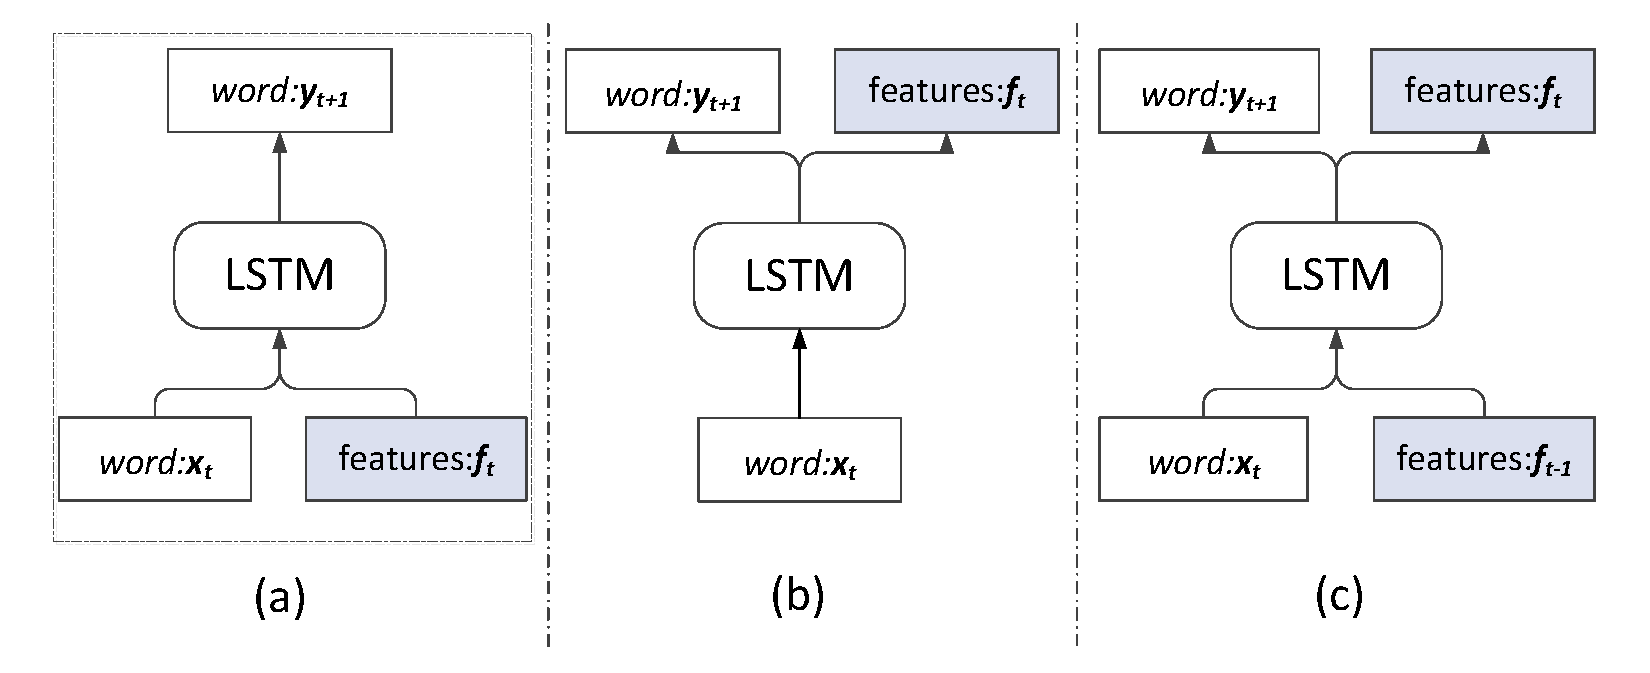
\includegraphics[width=\linewidth]{struclm/LSTM.pdf}
    \caption{{\it (a)Multi-view LSTM语言模型. (b)Multi-task LSTM语言模型. (c)Joint train LSTM语言模型.}}
    \label{fig:LSTM}
  \end{figure}
\subsection{Multi-task语言模型}
正如图\ref{fig:LSTM}$(b)$所展示的, 在Multi-task模型结构中,语言模型被设计成和其它的模型一起训练。
它们共享输入和一部分的隐层\cite{Collobert2008A}, 

However most researches on multi-task structure show that usually performance gain is achieved in the cooperating task, instead of LM task itself.


\subsection{multi-task模型结构}
\subsection{multi-task语言模型的表现}

\subsection{Multi-view语言模型}
Considering that some extra linguistic features might contribute to  language modeling, word and sentence level features were introduced in LM \cite{shi2012towards}. This model have multi inputs, which contains different views of information. So it is called multi-view model (see \ref{fig:LSTM}$(a)$).

As argued in Section 1, research on this kind of model shows improvements on perplexity and word prediction accuracy (WPA), but integrating this model with ASR did not lead to commensurate improvements \cite{shi2015integrating}.
That is to say, the straightforward combination of words and features as the inputs of a language model do not contribute to speech recognition.

Our proposed model is based on the multi-view structure, but is specially tailored for ASR task by using word-synchronized auxiliary feature.

\subsubsection{multi-view语言模型的结构}
\subsubsection{multi-view的多视角特征信息介绍}
\subsubsection{multi-view语言模的表现}

\subsection{Joint-train语言模型}
Other works combined the multi-task structure with multi-view structure, which is shown in Figure~\ref{fig:LSTM}$(c)$. Not only multiple tasks were trained together, but also the inputs of this model were multi-view. LM was jointed with other spoken language understanding (SLU) or natural language process (NLP) task, some models of improved version are researched. Better than multi-task models, these works show slight improvement in PPL and ASR-rescoring, but more promotion is gained in the cooperating task \cite{Liu2016Joint}.


\subsubsection{Joint-train语言模型结构}
\subsection{研究动机和思路}
我们猜测造成上述现象的主要原因是因为那些额外的辅助信息用的都是标准的标注算法,比如最大熵算法和双向LSTM模型,这些模型虽然表现优秀,但是在标注过程中用到了全局信息。
也就是不仅用到了前文的信息,更用到了后文的信息。
这就意味着在训练语言模型的时候,给当前词的辅助信息中包含后文信息,然后语言模型再用后文信息去预测后面的词。有点类似于信息作弊的感觉。这也是为什么在PPL任务上表现优秀的原因。

那为什么又在重打分任务中没有提升呢,这可能是因为重打分任务中的n-best集合(在第四章实验部分详细介绍)中的各种句子是本身就不合理的(语言模型得分很低),用不合理的后文信息得到的标注也会存在问题。
也就是意味着用不合理的后文信息预测后面的词,自然会出现偏差。

为了验证和解决这个问题,为了使得结构化语言模型不仅提升了语言模型的某个指标(PPL),更是要使得它在实际应用中(ASR任务)中有所提升,我们提出仅仅使用单向的辅助信息去训练结构化的语言模型。

基于这个思想,我们进行了一系列研究工作。
在我们的工作中,我们使用一个单向LSTM标注模型去进行双向信息的单向化。保证从词模型中出来的标注信息仅仅会包含历史信息,而不包含未来信息。
紧接着,标注模型的输入被作为Multi-view语言模型的一个输入接入到一个LSTM语言模型结构中。
在这种模型结构下,存在不同的训练方法,我们总共尝试了五种不同的训练方法。
最后我们将我们提出的模型和前人的相似结构模型进行多方位的在PPL和ASR任务上的比较。
%%%%%%%%%%%%%%%%%%%%%%%%%%%%%%%%%%%%%%%%%%%%%%%%%%%%%%%%%%%%%%%%%%%%%

\section{单向辅助信息模型的辅助信息选取}
\subsection{词性标注} 
词性是用来表示一个词的性质的,例如名词、形容词、动词等,每个词都有词性,有的甚至不止一种词性,根据在句子中所扮演的成分不同而有区别。

词性标注(Part-Of-Speech Tagger,POS Tagger)为以前无限的语言模型提供了有限的句法信息,例如限定词往往紧随其后的是名词。此外,对语言模型添加词性标记可以被看作是一种平滑,对于那种在训练数据中出现概率很小的单词,加入词性的语言模型相当于给他们分配了更一般的抽象类,从而增大他们的概率使其不再接近于0,从而可以更好的处理它们[20]。
词性标注是自然语言处理(NLP,Natural Language Processing)的范畴,

词性标注任务研究如何判别一个句子中的每个词的词性类别,如名词、动词、形容词等。
词性是最基础也最常用的一类特征。
在大量涉及自然语言的应用,如语音合成、句法分析、机器翻译中,词性都是必不可少的输入特征,其识别结果的正确性对这些系统的最终表现也有着显著的影响。
词性标注是一个典型的标注任务,它的输入为一串词序列,每个词所对应的词性即为输出,如图\ref{fig:possample}所示,


 \begin{figure}[tbhp!]
    \small
    \centering
    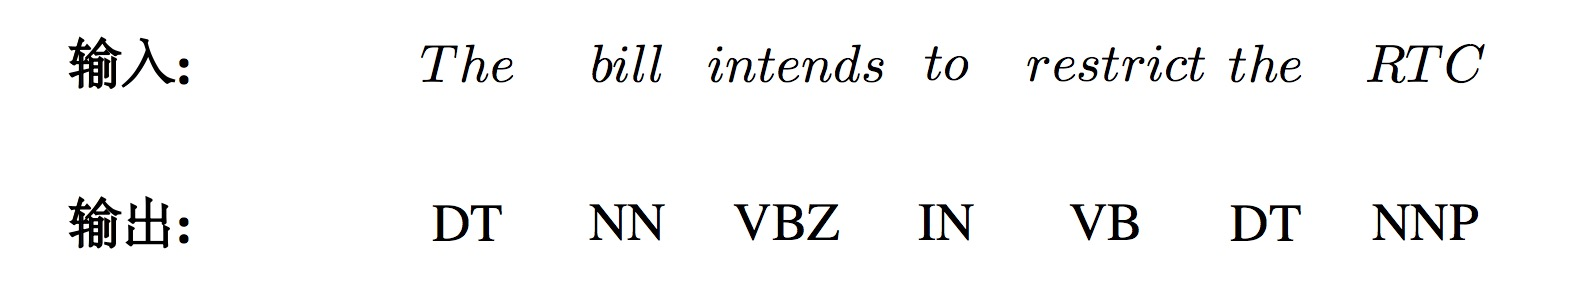
\includegraphics[width=\linewidth]{struclm/possam.jpeg}
    %\caption{{\it (a)Multi-view LSTM语言模型. (b)Multi-task LSTM语言模型. (c)Joint train LSTM语言模型.}}
    \caption[词性标注任务输入输出示例]{\textbf{词性标注任务输入输出示例。}输入为词序列(即句子),输出为该句子的词性标注序列。}
    \label{fig:fpossample}
  \end{figure}

本文采用的词性标注工具是斯坦福大学的开源词性标注工具,具有各种语言之分。输入到词性标注工具中的文本是已经经过分词处理的中文文本,若是英文文本可以直接进行词性标记,没有分词这个步骤。每个词的词性并不是固定的,例如“游泳”既可以是动词,也可以是名词,具体标记的算法由词性标记工具实现。

获得词性标注之后,我们用处理词向量的方式来处理词性标注。同样我们建立一个词性的词表,对于每一个词性,将其映射到词表上,对应的位置为$1$,其它为$0$,最后得到的就是一个一维的长度为词性的个数,对应位置为$1$其它为$0$的向量,如公式

\begin{equation}
    {pos_t}(i)=\left\{  
             \begin{array}{lr}  
             1  ({wp_t} = {vp_i}) \\
             0  ({wp_t} \not= {vp_i}) 
             \end{array}  
	\right.  
\end{equation}

其中${pos_t}$ 为当前$t$时刻的单词对应的词性所表示的向量,$i$表示向量的第$i$维, ${wp_t}$表示当前的单词所对应的词性, ${vp_i}$表示词性的词表中第$i$个词性。它即是词性的特征向量。

\subsection{命名实体识别} 
命名实体识别(Named Entity Recognition,简称NER),又称作“专名识别”,是指识别文本中具有特定意义的实体,主要包括人名、地名、机构名、专有名词等。
命名实体识别也是信息抽取(Information Extraction)相关任务的核心技术,因此有着很高的研究价值。
通常包括两部分:(1)实体边界识别;(2) 确定实体类别(人名、地名、机构名或其他)。英语中的命名实体具有比较明显的形式标志(即实体中的每个词的第一个字母要大写),所以实体边界识别相对容易,任务的重点是确定实体的类别。和英语相比,汉语命名实体识别任务更加复杂,而且相对于实体类别标注子任务,实体边界的识别更加困难。


与语块切分类似,命名实体识别也是一个切分任务,同样可以使用IOBES的标注策略转化为标准标注任务,输入输出样例如图\ref{fig:nersample}所示。

\begin{figure}[tbhp!]
\small
\centering
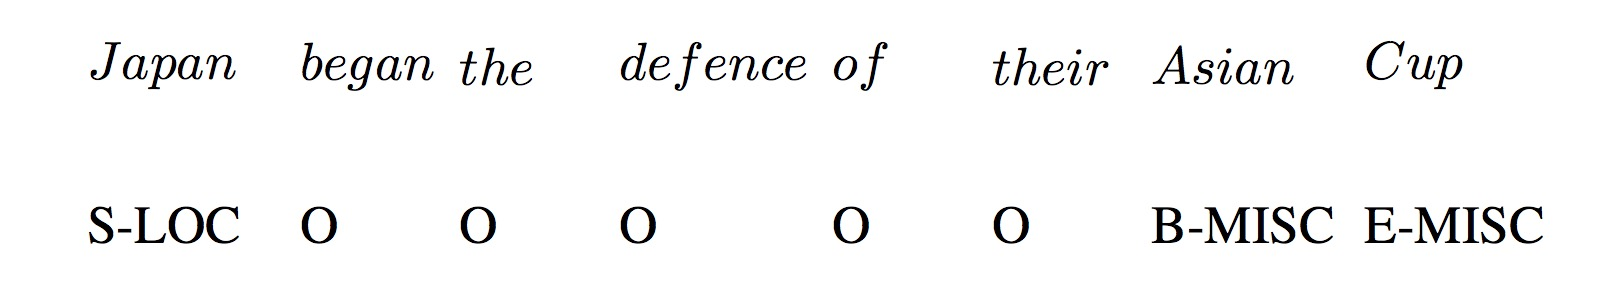
\includegraphics[width=\linewidth]{struclm/nersam.jpeg}
%\input{struclm/graph.nersample.tex}
\caption[命名实体识别任务输入输出示例]{\textbf{命名实体识别任务输入输出示例。}输入为词序列,输出为该句子的命名实体识别标签序列(使用了IOBES标注策略)。}\label{fig:nersample}
\end{figure}



\subsection{语法块标注} 
语块切分任务也称为浅层句法分析(shallow parsing),它研究如何把句子切分成不同的句法模块,如名词词组(Noun Phrase,NP)、动词词组(Verb Phrase,VP)、介词词组(Preposition Phrase,PP)等。
与词性标注类似,语块切分同样也是一种常用且重要的特征,对于句法分析、语义理解任务尤其重要。
与词性标注不同,语块切分是一个分割(segmentation)任务。
分割任务需要明确指定当前词所属类别的边界,边界内的词都属于同一类别,简单套用本章开头定义的标注模型不能确保上述限制条件。
不过通过使用特定的标注策略如IOBES、IOB、IOE等,语块切分任务也可以转成一个标准的标注任务。

以IOBES标注策略为例,该标注策略将每个原有的类别X扩展成四个子类别B-X,I-X,E-X与S-X,每个子类分别表示当前词属于$X$类且处于分割的开始位置(\textbf{B}egin),中间位置(\textbf{I}ntermediate),结尾(\textbf{E}nd)与单词分割(\textbf{S}ingle)。
此外,该策略还额外引入标签$O$表示该标签不属于任何分割(\textbf{O}ther)。
使用该标注策略的语块切分系统,首先预测每个词的IOBES扩展后的子类别,然后以$B$,$E$,$S$,$O$为边界将输出切分成段。
使用IOBES策略的输出与切分结果示例如图\ref{fig.tagschemesample}所示。
\begin{figure}[tbhp!]
\small
\centering
%\input{struclm/graph.chunksam1.jpeg}
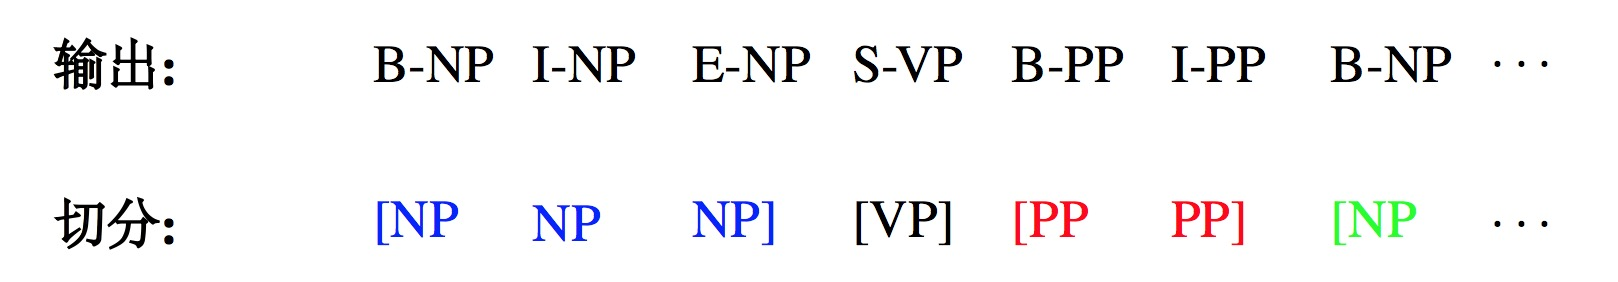
\includegraphics[width=\linewidth]{struclm/chunksam1.jpeg}
\caption[IOBES标注策略输出与切分示例]{\textbf{IOBES标注策略输出与切分示例。}}\label{fig.tagschemesample}
\end{figure}

IOB,IOE与IOBES类似,只是更加简化只有三个子类。
表\ref{table.tagscheme}展示比较了上述三类标注策略。
\begin{table}
\centering
\begin{tabular}{|c|c|c|c|c|c|}
\hline
Scheme & Begin & Inside & End & Single & Other \\
\hline
IOB & B-X & I-X & I-X & B-X & O \\
\hline
IOE & I-X & I-X & E-X & E-X & O \\
\hline
IOBES & B-X & I-X & E-X & S-X & O \\
\hline
\end{tabular}
\caption[IOB,IOE,IOBES标注策略比较]{\textbf{IOB,IOE,IOBES标注策略比较。}}\label{table.tagscheme}
\end{table}
在实际应用中,这三种标注方式都有工作使用,关于他们的优劣目前也无定论。
本文选择使用IOBES策略。
关于语块切分的输入输出样例如图\ref{fig.chunksample}所示。
\begin{figure}[tbhp!]
\small
\centering
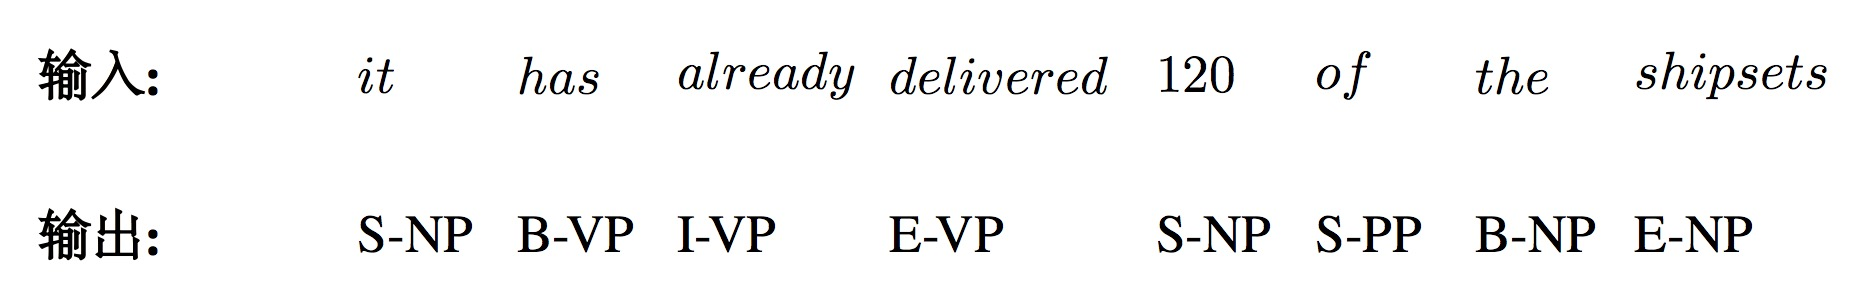
\includegraphics[width=\linewidth]{struclm/chunksam2.jpeg}
%\input{struclm/chunksam2.jpeg}
\caption[语块切分任务输入输出示例]{\textbf{语块切分任务输入输出示例。}输入为词序列,输出为该句子的语块切分标签序列(使用了IOBES标注策略)。}\label{fig.chunksample}
\end{figure}



\section{单向辅助信息的Multi-view语言模型结构}
\label{Multi-view}
我们的模型总共由两个部分组成:第一部分是用来生成单向辅助信息特征的标注模型;另一个是一个和标注模型链接在一起的Multi-view语言模型。
对于这两个模型,我们都是用的单层单向LSTM模型,并且将这两个模型以此层面的粒度链接在一起。关于模型的详细介绍和数学基础将在下文给出。


\subsection{单向LSTM标注模型部分}
\label{sec:psd-ac-conf}
标注模型是一种分类模型,一个标注模型是通过训练得到为每个输入序列找到它所属类别并输出。
神经网络现在被广泛用于各种标注模型中\cite{schmid1994part},因为它能大幅图提升传统统计学标注模型的性能。
其中双向神经网络更为普遍\cite{Wang2015A},由于前后文信息的紧密结合,更是使得标注模型进一步提升。
神经网络的标注模型是根据输入输出它所属的类别的概率分布。



  \begin{figure}[tbhp!]
    \small
    \centering
    %\tikzset{
label/.style={
  rectangle,
  draw=none,
  text centered,
  inner sep=0.6em,
},
namelabel/.style={
  rectangle,
  draw=none,
  text width=12em,
  inner sep=0.6em,
  align=left
},
bigcircle/.style={
  rectangle,
  rounded corners,
  draw,
  minimum width=3em,
  text centered,
  inner sep=0.3em,
}
}

\scriptsize
\begin{tikzpicture}[x=1em, y=1em, >=stealth]
%nodes
\node[bigcircle](fht1) at (-5.5,0){LSTM};
\node[bigcircle](fht2) at (0,0){LSTM};
\node[bigcircle](fht3) at (5.5,0){LSTM};

\node[label](x0) at (-9,-4){$\dots$};
\node[label](x1) at (-5.5,-4){\underline{$w_{t-1}$}};
\node[label](x2) at (0,-4){\underline{$w_{t}$}};
\node[label](x3) at (5.5,-4){\underline{$w_{t+1}$}};
\node[label](x4) at (9,-4){$\dots$};

\node[label](y0) at (-9,4){$\dots$};
\node[label](y1) at (-5.5,4){\underline{$f_{t-1}$}};
\node[label](y2) at (0,4){\underline{$f_{t}$}};
\node[label](y3) at (5.5,4){\underline{$f_{t+1}$}};
\node[label](y4) at (9,4){$\dots$};

\node[namelabel](textoutputs) at (-14,4){Outputs:};
\node[namelabel](textbklayer) at (-14,0){Hidden Layer(LSTM):};
\node[namelabel](textinputs) at (-14,-4){Inputs:};

\draw[->](fht1) to (y1);
\draw[->](fht2) to (y2);
\draw[->](fht3) to (y3);

\draw[->] (-10,0) -- (fht1);
\draw[->](fht1) -- (fht2);
\draw[->](fht2) -- (fht3);
\draw[->](fht3) -- (10,0);

\draw[->] (x1) -- (fht1);
\draw[->] (x2) -- (fht2);
\draw[->] (x3) -- (fht3);


\end{tikzpicture}

    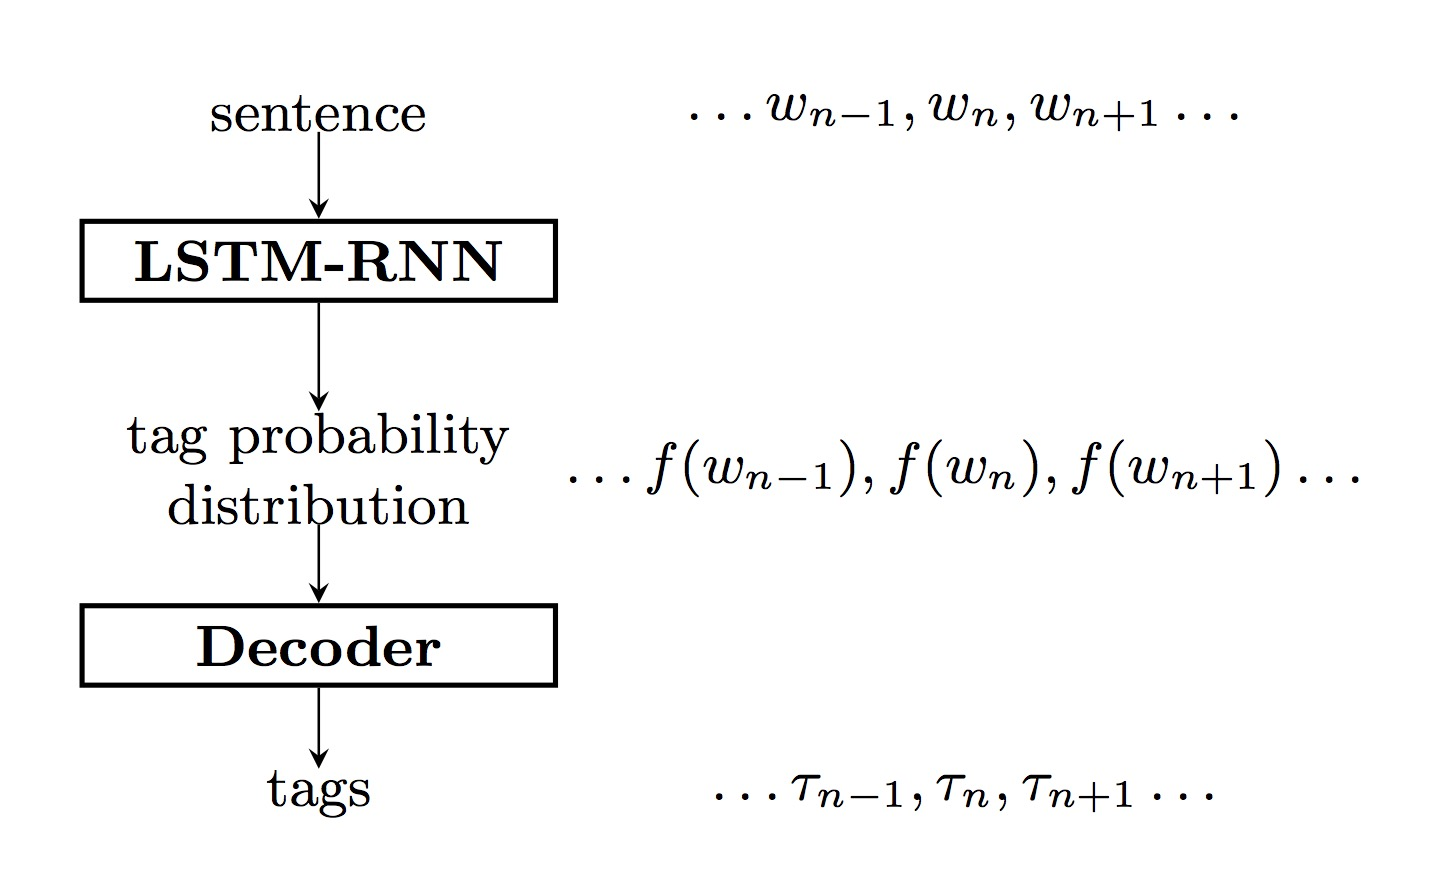
\includegraphics[width=\linewidth]{struclm/tagging.jpeg}
    \caption{{\it uni-directional LSTM tagging model}}
    \label{fig:tagging}
  \end{figure}

不过如前文所说,本文这里必须使用单向神经网络。
另外在我们的验证实验和我们的三种标注任务中,双向LSTM模型相比于相同参数的单向LSTM模型仅仅有非常微小的性能提升。
如图\ref{fig:tagging}所示,这是一个单向模型的模型结构示意图,
一个LSTM网络结构就和RNN一样有隐层的递归的自环,其中每个隐层单元被替换成了具有长短时记忆功能的LSTM单元。
在后文中,LSTM记忆单元被统一表示成$\mathcal{L}$。另外为了避免混淆,标注模型和语言模型的LSTM记忆单元分别被表示成 $\mathcal{L}_{\tt{tag}}$和$\mathcal{L}_{\tt{LM}}$。



向量$\bm{w}_t$使用one hot编码来表示当前时刻$t$的当前词,这个one hot向量也同时是$\mathcal{L}_{\tt{tag}}$和$\mathcal{L}_{\tt{LM}}$.

接下来,这个词的此嵌套$\bm{x}_t$可以这样得到:
	\begin{equation}
    \bm{x}_t = E_{tag}\bm{w}_t
	\end{equation}
这里$E_{tag}$ 是指标注模型的词嵌套矩阵。    

单向LSTM标注模型的输出层 $\bm{h}_t$ 由下述公式计算得到:  
	\begin{equation}
    \bm{h}_t = \mathcal{L}_{\tt{tag}}(\bm{x}_t,\bm{h}_{t-1})
	\end{equation}
其中LSTM计算单元$\mathcal{L}$内部的详细的函数表达式如公式ref{eq:memoryb}所展示的这样:

其中 $\sigma$ 是逻辑函数 (sigmoid), 以及$i$, $f$, $o$ and $c$ 分别表示 \textit{input gate}、 \textit{forget gate}、 \textit{output gate} and \textit{cell} 激励向量.



$\bm{f}_t$ 是标注模型的输出,这是个总和为$1$的向量,表示输出的标注分类的概率分布, 同样的它可以根据模型的隐层LSTM记忆单元求得,公式如下:
	\begin{equation}
    \bm{f}_t = softmax(W_{ho}\bm{h}_{t}+\bm{b}_y)
	\end{equation}	
其中softmax是归一化函数,目的是让概率分布总和为1.




 %and vector $\mathbf{s}(t-1)$ represents the hidden layer output in the previous time step.
根据截止到目前所描述的LSTM-RNN语言模型,观测到的每个时刻的模型的输出概率分布和其它时刻是相互独立的,仅仅根据数据训练得出。
然而,在有些任务中,比如说NER和Chunking任务中,标注之间具有一些隐含的规则,它们之间和前后的标注具有强关联性。其中一部分种类仅仅能存在在部分特定的种类之后,而一部分不能存在于某些之后。比如说NN-B(名字块开头)后面不可能跟VV-E(动词块)结尾,加了类似于这些规则之后标注模型的准确率会有一定的提升。


为了将上述的标注之间的约束关系利用起来,
我们在每一步中引入转化矩阵的概念,如果两个标注类别之间可以连接,则矩阵为1,否则为0。矩阵是单向的,比如B能在A后面出现,则$matrix[A][B]=0$,而B不一定能在A之前出现,若不能则$matrix[B][A]=0$。
这个矩阵和标注模型的概率分布一起进行解码\cite{Wang2015A},便能得到概率最大的标注序列。 
这个解码过程可以用经典的Viterbi算法\cite{Andrew1967Viterbi}完成。

在本文中,解码过程被表示成$\mathcal{D}(\cdot)$,
解码过程的输出$\mathbf{\tau}_t$ 是一系列最终预测得到的标注序列,它们同样用one hot向量表示如下:

	\begin{equation}
    \bm{\tau}_t = \mathcal{D}(\bm{f}_t)
	\end{equation}

到此我们可以发现,标注模型的输出传到语言模型中可以有两种表示:第一种是概率分布的序列,第二种是经过Viterbi解码后得到的确切的one hot序列。



\subsection{Multi-view语言模型部分}
\label{sec:psd-ac-conf}
图\ref{fig:selfpos} 展现了我们的仅用前文辅助信息的Multi-view LSTM语言模型架构。

  \begin{figure}[tbhp!]
    \small
    \centering
    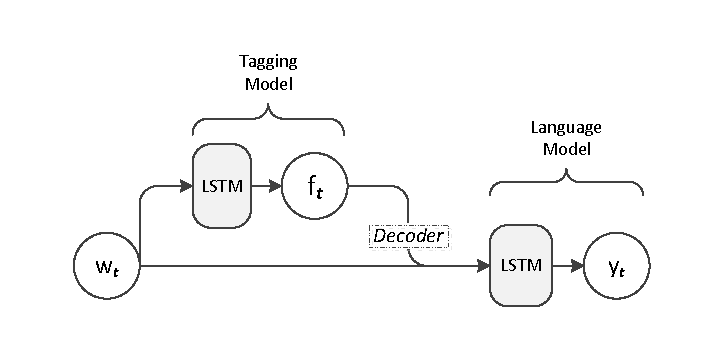
\includegraphics[width=\linewidth]{struclm/selfpos.pdf}
    \caption{{\it multi-view LSTM  language model with word-synchronized auxiliary feature}}
    \label{fig:selfpos}
  \end{figure}


我们提出的模型是一个和单向标注模型连接起来的Multi-view语言模型。

语言模型的第一个输入 $\bm{w}_t$ 是一个代表当前词的one hot向量 , 这个向量同时也是标注模型的输入。
第二个输入是标注模型部分的输出,可以是经过Viterbi解码之后的ont序列,也可以是直接的概率分布。
无论这个解码过程有没有进行,我都对于两者都在第四章的实验部分进行了实验与比较。
它们的不同点也体现在输入部分的公式上,
如果使用了Viterbi解码,语言模型的第二个输入将会是:
	\begin{equation}
\bm{\zeta}_t=W_{tag}\bm{\tau}_t + E_{word}\bm{w}_t 
	\end{equation}
其中$\bm{\tau}_t$ 是解码部分输出的one hot向量。
否则,语言模型的输入是:
	\begin{equation}
\bm{\zeta}_t=W_{tag}\bm{f}_t +  E_{word}\bm{w}_t 
	\end{equation} 
其中$\bm{f}_t$ 是标注模型的概率分布形式的输出。
$E_{word}$ is 是词嵌套矩阵,$W_{tag}$ 是标注模型到语言模型的隐层之间的参数矩阵。它们将会在每个时序点被加起来作为语言模型最终的输入。



%The same as tagging model, as $\bm{\sigma}_t$ is the input of $\mathcal{L}_{\tt{LM}}$.
LSTM语言模型的隐层的输出为 $\bm{h}_t$,它的计算公式是: 
	\begin{equation}
    \bm{h}_t = \mathcal{L}_{\tt{LM}}(\bm{\zeta}_t,\bm{h}_{t-1})
	\end{equation}
LSTM记忆快的具体函数 $\mathcal{L}$ 的公式已经在上一小节介绍过了。
$\bm{y}_{t}$ 是语言模型的输出,
表示预测的下一个词的概率分布$P(\bm{x}_{t+1}|\bm{x}_1\mathord{:}\bm{x}_t)$, 
它同样根据LSTM隐层单元得到,公式如下: 
	\begin{equation}
    \bm{y}_{t} = softmax(W_{ho}\bm{h}_{t}+\bm{b}_y)
	\end{equation}	
    
上述就我我们单向自信息Multi-view语言模型的结构描述。
    
\section{模型的训练方法}
我们提出的模型由两部分组成:标注模型和语言模型。
语言模型训练过程遵循标准约定,先计算每个单词的交叉熵,然后进行反向传播。
我们采用基于小批量的随机梯度下降法(SGD)作为优化方法。
但是由于语言模型和标注模型的连接方式的不同,我们尝试了五种不同的训练方法,并进行实验和比较。
五种训练方式如下:

1) 将LSTM标记模型作为一个独立的模型进行训练,在训练多视角语言模型时将标注模型固定,并不继续进行训练更新。五种方式中只有这种方法才能利用解码过程,因为后面的方法需要训练标注模型,但解码过程出来的结果是确定的值,无论是解码还是采样过后都不支持将误差从语言模型传递到标注模型,从而不支持继续训练标注模型。其优势在于,解码器有利于提升标注模型,但它的缺点是在语言模型训练时标注模型不能更新。

2)提前对LSTM标注模型进行训练,不同于第一种方法,这种方法中标注模型也会在训练语言模型的时候进行训练和更新,此时标注模型的输出是以概率分布的形式输入到语言模型中。标注模型的学习率下降速度和语言模型保持一致。这个方法有个致命缺点是:训练好的标注模型会因为不恰当的学习率在训练语言模型的时候训毁。

3)并不事先训练好标注模型,而是对其进行随机初始化,然后整个系统——标注模型和语言模型部分一起记性训练,使用相同的学习率。 


4)第三种和第四种方式都是实用的相同学习率,本方法在第二种训练方法的基础上,采用学习率稳定算子$\beta$自适应算法 \cite{Ghahremani2016Self}\cite{Liu2016investigation} 进行模型的更新,目的是为了合理的调整学习旅使得在不同的模型部分使用适合于它自己的学习率。比如第二种方法中标注模型是事先训练好的, 调整幅度就应该非常小。 

5)与第四种方式相似, 这个方法是在第三种方法的基础上加入稳定算子$\beta$自适应算法。

由于我们所提出的模型的最佳训练方法是未知的,所以这五种方法都在实验中进行了测试和评估。结果如第$4$章实验部分所示。







%# -*- coding: utf-8-unix -*-
%%==================================================
%% chapter02.tex for SJTU Master Thesis
%% based on CASthesis
%% modified by wei.jianwen@gmail.com
%% Encoding: UTF-8
%%==================================================

\chapter{ \LaTeX 实验与分析}
\label{chap:experiment}

\section{实验设计}
\label{sec:exp_desg}

\section{实验准备}
\label{sec:exp_pre}

\section{实验结果}
\label{sec:exp_res}
以下是一个无序列表的例子,列表的每个条目单独分段。

\begin{itemize}
  \item 这是一个无序列表。
  \item 这是一个无序列表。
  \item 这是一个无序列表。
\end{itemize}

使用\verb+itemize*+环境可以创建行内无序列表。
\begin{itemize*}
  \item 这是一个无序列表。
  \item 这是一个无序列表。
  \item 这是一个无序列表。
\end{itemize*}
行内无序列表条目不单独分段,所有内容直接插入在原文的段落中。

\subsection{有序列表}
\label{sec:orderlist}

使用环境\verb+enumerate+和\verb+enumerate*+创建有序列表,
使用方法无序列表类似。

\begin{enumerate}
  \item 这是一个有序列表。
  \item 这是一个有序列表。
  \item 这是一个有序列表。
\end{enumerate}

使用\verb+enumerate*+环境可以创建行内有序列表。
\begin{enumerate*}
  \item 这是一个默认有序列表。
  \item 这是一个默认有序列表。
  \item 这是一个默认有序列表。
\end{enumerate*}
行内有序列表条目不单独分段,所有内容直接插入在原文的段落中。

\subsection{描述型列表}

使用环境\verb+description+可创建带有主题词的列表,条目语法是\verb+\item[主题] 内容+。
\begin{description}
    \item[主题一] 详细内容
    \item[主题二] 详细内容
    \item[主题三] 详细内容 \ldots
\end{description}

\subsection{自定义列表样式}

可以使用\verb+label+参数控制列表的样式,
详细可以参考WikiBooks\footnote{\url{https://en.wikibooks.org/wiki/LaTeX/List_Structures\#Customizing_lists}}。
比如一个自定义样式的行内有序列表
\begin{enumerate*}[label=\itshape\alph*)\upshape]
  \item 这是一个自定义样式有序列表。
  \item 这是一个自定义样式有序列表。
  \item 这是一个自定义样式有序列表。
\end{enumerate*}

\section{数学排版}
\label{sec:matheq}

\subsection{公式排版}
\label{sec:eqformat}

这里有举一个长公式排版的例子,来自\href{http://www.tex.ac.uk/tex-archive/info/math/voss/mathmode/Mathmode.pdf}{《Math mode》}:

\begin {multline}
  \frac {1}{2}\Delta (f_{ij}f^{ij})=
  2\left (\sum _{i<j}\chi _{ij}(\sigma _{i}-
    \sigma _{j}) ^{2}+ f^{ij}\nabla _{j}\nabla _{i}(\Delta f)+\right .\\
  \left .+\nabla _{k}f_{ij}\nabla ^{k}f^{ij}+
    f^{ij}f^{k}\left [2\nabla _{i}R_{jk}-
      \nabla _{k}R_{ij}\right ]\vphantom {\sum _{i<j}}\right )
\end{multline}

\subsection{SI单位}

使用\verb+siunitx+宏包可以方便地输入SI单位制单位,例如\verb+\SI{5}{\um}+可以得到\SI{5}{\um}。

\subsubsection{一个四级标题}
\label{sec:depth4}

这是全文唯一的一个四级标题。在这部分中将演示了mathtools宏包中可伸长符号(箭头、等号的例子)的例子。

\begin{displaymath}
    A \xleftarrow[n=0]{} B \xrightarrow[LongLongLongLong]{n>0} C 
\end{displaymath}

\begin{eqnarray}
  f(x) & \xleftrightarrow[]{A=B}  & B \\
  & \xleftharpoondown[below]{above} & B \nonumber \\
  & \xLeftrightarrow[below]{above} & B
\end{eqnarray}

又如:

\begin{align}
  \label{eq:none}
  & I(X_3;X_4)-I(X_3;X_4\mid{}X_1)-I(X_3;X_4\mid{}X_2) \nonumber \\
  = & [I(X_3;X_4)-I(X_3;X_4\mid{}X_1)]-I(X_3;X_4\mid{}\tilde{X}_2) \\
  = & I(X_1;X_3;X_4)-I(X_3;X_4\mid{}\tilde{X}_2)
\end{align}

\subsection{定理环境}

模板中定义了丰富的定理环境
algo(算法),thm(定理),lem(引理),prop(命题),cor(推论),defn(定义),conj(猜想),exmp(例),rem(注),case(情形),
bthm(断言定理),blem(断言引理),bprop(断言命题),bcor(断言推论)。
amsmath还提供了一个proof(证明)的环境。
这里举一个“定理”和“证明”的例子。
\begin{thm}[留数定理]
\label{thm:res}
  假设$U$是复平面上的一个单连通开子集,$a_1,\ldots,a_n$是复平面上有限个点,$f$是定义在$U\backslash \{a_1,\ldots,a_n\}$上的全纯函数,
  如果$\gamma$是一条把$a_1,\ldots,a_n$包围起来的可求长曲线,但不经过任何一个$a_k$,并且其起点与终点重合,那么:

  \begin{equation}
    \label{eq:res}
    \ointop_{\gamma}f(z)\,\mathrm{d}z = 2\uppi\mathbf{i}\sum^n_{k=1}\mathrm{I}(\gamma,a_k)\mathrm{Res}(f,a_k)
  \end{equation}

  如果$\gamma$是若尔当曲线,那么$\mathrm{I}(\gamma, a_k)=1$,因此:

  \begin{equation}
    \label{eq:resthm}
    \ointop_{\gamma}f(z)\,\mathrm{d}z = 2\uppi\mathbf{i}\sum^n_{k=1}\mathrm{Res}(f,a_k)
  \end{equation}

      % \oint_\gamma f(z)\, dz = 2\pi i \sum_{k=1}^n \mathrm{Res}(f, a_k ). 

  在这里,$\mathrm{Res}(f, a_k)$表示$f$在点$a_k$的留数,$\mathrm{I}(\gamma,a_k)$表示$\gamma$关于点$a_k$的卷绕数。
  卷绕数是一个整数,它描述了曲线$\gamma$绕过点$a_k$的次数。如果$\gamma$依逆时针方向绕着$a_k$移动,卷绕数就是一个正数,
  如果$\gamma$根本不绕过$a_k$,卷绕数就是零。

  定理\ref{thm:res}的证明。
  
  \begin{proof}
    首先,由……

    其次,……

    所以……
  \end{proof}
\end{thm}

上面的公式例子中,有一些细节希望大家注意。微分号d应该使用“直立体”也就是用mathrm包围起来。
并且,微分号和被积函数之间应该有一段小间隔,可以插入\verb+\,+得到。
斜体的$d$通常只作为一般变量。
i,j作为虚数单位时,也应该使用“直立体”为了明显,还加上了粗体,例如\verb+\mathbf{i}+。斜体$i,j$通常用作表示“序号”。
其他字母在表示常量时,也推荐使用“直立体”譬如,圆周率$\uppi$(需要upgreek宏包),自然对数的底$\mathrm{e}$。
不过,我个人觉得斜体的$e$和$\pi$很潇洒,在不至于引起混淆的情况下,我也用这两个字母的斜体表示对应的常量。


\section{向文档中插入图像}
\label{sec:insertimage}

\subsection{支持的图片格式}
\label{sec:imageformat}

\XeTeX 可以很方便地插入PDF、PNG、JPG格式的图片。

插入PNG/JPG的例子如\ref{fig:SRR}所示。
这两个水平并列放置的图共享一个“图标题”(table caption),没有各自的小标题。

\begin{figure}[!htp]
  \centering
  \includegraphics[width=0.3\textwidth]{example/sjtulogo.png}
  \hspace{1cm}
  \includegraphics[width=0.3\textwidth]{example/sjtulogo.jpg}
  \bicaption[fig:SRR]{这里将出现在插图索引中}{中文题图}{Fig}{English caption}
\end{figure}

% 这里还有插入eps图像和pdf图像的例子,如图\ref{fig:epspdf:a}和图\ref{fig:epspdf:b}。这里将EPS和PDF图片作为子图插入,每个子图有自己的小标题。并列子图的功能是使用subfigure宏包提供的。
% 
% \begin{figure}
%   \centering
%   \subfigure[EPS Figure]{
%     \label{fig:epspdf:a} %% label for first subfigure
%     \includegraphics[width=0.3\textwidth]{example/sjtulogo.eps}}
%   \hspace{1in}
%   \subfigure[PDF Figure]{
%     \label{fig:epspdf:b} %% label for second subfigure
%     \includegraphics[width=0.3\textwidth]{example/sjtulogo.pdf}}
%   \bicaption[fig:pdfeps]{插入eps图像和pdf图像}{插入eps和pdf的例子}{Fig}{An EPS and PDF demo}
% \end{figure}

更多关于 \LaTeX 插图的例子可以参考\href{http://www.cs.duke.edu/junhu/Graphics3.pdf}{《\LaTeX 插图指南》}。

\subsection{长标题的换行}
\label{sec:longcaption}

图\ref{fig:longcaptionbad}和图\ref{fig:longcaptiongood}都有比较长图标题,通过对比发现,图\ref{fig:longcaptiongood}的换行效果更好一些。
其中使用了minipage环境来限制整个浮动体的宽度。

\begin{figure}[!htp]
 \centering
 \includegraphics[width=4cm]{example/sjtulogo.pdf}
 \bicaption[fig:longcaptionbad]{这里将出现在插图索引}{海交通大学是我国历史最悠久的高等学府之一,是教育部直属、教育部与上海市共建的全国重点大学.}{Fig}{Where there is a will, there is a way.}
\end{figure}

\begin{figure}[!htbp]
  \centering
  \begin{minipage}[b]{0.6\textwidth}
    \captionstyle{\centering}
    \centering
    \includegraphics[width=4cm]{example/sjtulogo.pdf}
    \bicaption[fig:longcaptiongood]{这里将出现在插图索引}{海交通大学是我国历史最悠久的高等学府之一,是教育部直属、教育部与上海市共建的全国重点大学.}{Fig}{Where there is a will, there is a way.}
  \end{minipage}     
\end{figure}

\subsection{绘制流程图}

图\ref{fig:flow_chart}是一张流程图示意。使用tikz环境,搭配四种预定义节点(\verb+startstop+、\verb+process+、\verb+decision+和\verb+io+),可以容易地绘制出流程图。
\begin{figure}[!htp]
    \centering
    \resizebox{6cm}{!}{\input{figure/example/flow_chart.tex}}
    \bicaption[fig:flow_chart]{绘制流程图效果}{流程图}{Fig}{Flow chart}
\end{figure}
  
\clearpage

\section{表格}
\label{sec:tab}

这一节给出的是一些表格的例子,如表\ref{tab:firstone}所示。

\begin{table}[!hpb]
  \centering
  \bicaption[tab:firstone]{指向一个表格的表目录索引}{一个颇为标准的三线表格\footnotemark[1]}{Table}{A Table}
  \begin{tabular}{@{}llr@{}} \toprule
    \multicolumn{2}{c}{Item} \\ \cmidrule(r){1-2}
    Animal & Description & Price (\$)\\ \midrule
    Gnat & per gram & 13.65 \\
    & each & 0.01 \\
    Gnu & stuffed & 92.50 \\
    Emu & stuffed & 33.33 \\
    Armadillo & frozen & 8.99 \\ \bottomrule
  \end{tabular}
\end{table}
\footnotetext[1]{这个例子来自\href{http://www.ctan.org/tex-archive/macros/latex/contrib/booktabs/booktabs.pdf}{《Publication quality tables in LATEX》}(booktabs宏包的文档)。这也是一个在表格中使用脚注的例子,请留意与threeparttable实现的效果有何不同。}

下面一个是一个更复杂的表格,用threeparttable实现带有脚注的表格,如表\ref{tab:footnote}。

\begin{table}[!htpb]
  \bicaption[tab:footnote]{出现在表目录的标题}{一个带有脚注的表格的例子}{Table}{A Table with footnotes}
  \centering
  \begin{threeparttable}[b]
     \begin{tabular}{ccd{4}cccc}
      \toprule
      \multirow{2}{6mm}{total}&\multicolumn{2}{c}{20\tnote{1}} & \multicolumn{2}{c}{40} &  \multicolumn{2}{c}{60}\\
      \cmidrule(lr){2-3}\cmidrule(lr){4-5}\cmidrule(lr){6-7}
      &www & k & www & k & www & k \\
      \midrule
      &$\underset{(2.12)}{4.22}$ & 120.0140\tnote{2} & 333.15 & 0.0411 & 444.99 & 0.1387 \\
      &168.6123 & 10.86 & 255.37 & 0.0353 & 376.14 & 0.1058 \\
      &6.761    & 0.007 & 235.37 & 0.0267 & 348.66 & 0.1010 \\
      \bottomrule
    \end{tabular}
    \begin{tablenotes}
    \item [1] the first note.% or \item [a]
    \item [2] the second note.% or \item [b]
    \end{tablenotes}
  \end{threeparttable}
\end{table}

\section{参考文献管理}

 \LaTeX 具有将参考文献内容和表现形式分开管理的能力,涉及三个要素:参考文献数据库、参考文献引用格式、在正文中引用参考文献。
这样的流程需要多次编译:

\begin{enumerate}[noitemsep,topsep=0pt,parsep=0pt,partopsep=0pt]
	\item 用户将论文中需要引用的参考文献条目,录入纯文本数据库文件(bib文件)。
	\item 调用xelatex对论文模板做第一次编译,扫描文中引用的参考文献,生成参考文献入口文件(aux)文件。
	\item 调用bibtex,以参考文献格式和入口文件为输入,生成格式化以后的参考文献条目文件(bib)。
	\item 再次调用xelatex编译模板,将格式化以后的参考文献条目插入正文。
\end{enumerate}

参考文献数据库(thesis.bib)的条目,可以从Google Scholar搜索引擎\footnote{\url{https://scholar.google.com}}、CiteSeerX搜索引擎\footnote{\url{http://citeseerx.ist.psu.edu}}中查找,文献管理软件Papers\footnote{\url{http://papersapp.com}}、Mendeley\footnote{\url{http://www.mendeley.com}}、JabRef\footnote{\url{http://jabref.sourceforge.net}}也能够输出条目信息。

下面是在Google Scholar上搜索到的一条文献信息,格式是纯文本:

\begin{lstlisting}[caption={从Google Scholar找到的参考文献条目}, label=googlescholar, escapeinside="", numbers=none]
    @phdthesis{"白2008信用风险传染模型和信用衍生品的定价",
      title={"信用风险传染模型和信用衍生品的定价"},
      author={"白云芬"},
      year={2008},
      school={"上海交通大学"}
    } 
\end{lstlisting}

推荐修改后在bib文件中的内容为:

\begin{lstlisting}[caption={修改后的参考文献条目}, label=itemok, escapeinside="", numbers=none]
  @phdthesis{bai2008,
    title={"信用风险传染模型和信用衍生品的定价"},
    author={"白云芬"},
    date={2008},
    address={"上海"},
    school={"上海交通大学"}
  } 
\end{lstlisting}

按照教务处的要求,参考文献外观应符合国标GBT7714的要求\footnote{\url{http://www.cces.net.cn/guild/sites/tmxb/Files/19798_2.pdf}}。
在模板中,表现形式的控制逻辑通过bibla­tex-gb7714-2015包实现\footnote{\url{https://www.ctan.org/pkg/biblatex-gb7714-2015}},基于{Bib\LaTeX}管理文献。在目前的多数TeX发行版中,可能都没有默认包含biblatex-gb7714-2015,需要手动安装。

正文中引用参考文献时,用\verb+\cite{key1,key2,key3...}+可以产生“上标引用的参考文献”,
如\cite{Meta_CN,chen2007act,DPMG}。
使用\verb+\citen{key1,key2,key3...}+则可以产生水平引用的参考文献,例如\citen{JohnD,zhubajie,IEEE-1363}。
请看下面的例子,将会穿插使用水平的和上标的参考文献:关于书的\citen{Meta_CN,JohnD,IEEE-1363},关于期刊的\cite{chen2007act,chen2007ewi},
会议论文\citen{DPMG,kocher99,cnproceed},
硕士学位论文\citen{zhubajie,metamori2004},博士学位论文\cite{shaheshang,FistSystem01,bai2008},标准文件\citen{IEEE-1363},技术报告\cite{NPB2},电子文献\citen{xiaoyu2001, CHRISTINE1998},用户手册\citen{RManual}。

总结一些注意事项:
\begin{itemize}
\item 参考文献只有在正文中被引用了,才会在最后的参考文献列表中出现;
\item 参考文献“数据库文件”bib是纯文本文件,请使用UTF-8编码,不要使用GBK编码;
\item 参考文献条目中默认通过date域输入时间。兼容使用year域时会产生编译warning,可忽略。
\end{itemize}

\section{用listings插入源代码}

原先ctexbook文档类和listings宏包配合使用时,代码在换页时会出现莫名其妙的错误,后来经高人指点,顺利解决了。
感兴趣的话,可以看看\href{http://bbs.ctex.org/viewthread.php?tid=53451}{这里}。
这里给使用listings宏包插入源代码的例子,这里是一段C代码。
另外,listings宏包真可谓博大精深,可以实现各种复杂、漂亮的效果,想要进一步学习的同学,可以参考
\href{http://mirror.ctan.org/macros/latex/contrib/listings/listings.pdf}{listings宏包手册}。

\begin{lstlisting}[language={C}, caption={一段C源代码}]
#include <stdio.h>
#include <unistd.h>
#include <sys/types.h>
#include <sys/wait.h>

int main() {
  pid_t pid;

  switch ((pid = fork())) {
  case -1:
    printf("fork failed\n");
    break;
  case 0:
    /* child calls exec */
    execl("/bin/ls", "ls", "-l", (char*)0);
    printf("execl failed\n");
    break;
  default:
    /* parent uses wait to suspend execution until child finishes */
    wait((int*)0);
    printf("is completed\n");
    break;
  }

  return 0;
}
\end{lstlisting}

\section{用algorithm和algorithmicx宏包插入算法描述}

algorithmicx 比 algorithmic 增加了一些命令。
示例如算法\ref{algo:sum_100}和算法\ref{algo:merge_sort},
后者的代码来自\href{http://hustsxh.is-programmer.com/posts/38801.html}{xhSong的博客}。
algorithmicx的详细使用方法见\href{http://mirror.hust.edu.cn/CTAN/macros/latex/contrib/algorithmicx/algorithmicx.pdf}{官方README}。
使用算法宏包时,算法出现的位置很多时候不按照tex文件里的书写顺序, 
需要强制定位时可以使用\verb+\begin{algorithm}[H]+
\footnote{http://tex.stackexchange.com/questions/165021/fixing-the-location-of-the-appearance-in-algorithmicx-environment}

这是写在算法\ref{algo:sum_100}前面的一段话,在生成的文件里它会出现在算法\ref{algo:sum_100}前面。

\begin{algorithm}
% \begin{algorithm}[H] % 强制定位
\caption{求100以内的整数和}
\label{algo:sum_100}
\begin{algorithmic}[1] %每行显示行号
\Ensure 100以内的整数和 % 输出
\State $sum \gets 0$
\For{$i = 0 \to 100$}
    \State $sum \gets sum + i$
  \EndFor
\end{algorithmic}
\end{algorithm}

这是写在两个算法中间的一段话,当算法\ref{algo:sum_100}不使用\verb+\begin{algorithm}[H]+时它也会出现在算法\ref{algo:sum_100}前面。

对于很长的算法,单一的算法块\verb+\begin{algorithm}...\end{algorithm}+是不能自动跨页的
\footnote{http://tex.stackexchange.com/questions/70733/latex-algorithm-not-display-under-correct-section},
会出现的情况有:

\begin{itemize}
  \item 该页放不下当前的算法,留下大片空白,算法在下一页显示
  \item 单一页面放不下当前的算法,显示时超过页码的位置直到超出整个页面范围
\end{itemize}

解决方法有:

\begin{itemize}
  \item (推荐)使用\verb+algstore{algname}+和\verb+algrestore{algname}+来讲算法分为两个部分\footnote{http://tex.stackexchange.com/questions/29816/algorithm-over-2-pages},如算法\ref{algo:merge_sort}。
  \item 人工拆分算法为多个小的部分。
\end{itemize}

\begin{algorithm}
% \begin{algorithm}[H] % 强制定位
\caption{用归并排序求逆序数}
\label{algo:merge_sort}
\begin{algorithmic}[1] %每行显示行号
\Require $Array$数组,$n$数组大小 % 输入
\Ensure 逆序数 % 输出
\Function {MergerSort}{$Array, left, right$}
  \State $result \gets 0$
  \If {$left < right$}
    \State $middle \gets (left + right) / 2$
    \State $result \gets result +$ \Call{MergerSort}{$Array, left, middle$}
    \State $result \gets result +$ \Call{MergerSort}{$Array, middle, right$}
    \State $result \gets result +$ \Call{Merger}{$Array,left,middle,right$}
  \EndIf
  \State \Return{$result$}
\EndFunction
\State %空一行
\Function{Merger}{$Array, left, middle, right$}
  \State $i\gets left$
  \State $j\gets middle$
  \State $k\gets 0$
  \State $result \gets 0$
  \While{$i<middle$ \textbf{and} $j<right$}
    \If{$Array[i]<Array[j]$}
      \State $B[k++]\gets Array[i++]$
    \Else
      \State $B[k++] \gets Array[j++]$
      \State $result \gets result + (middle - i)$
    \EndIf
  \EndWhile
  \algstore{MergeSort}
\end{algorithmic}
\end{algorithm}

\begin{algorithm}
\begin{algorithmic}[1]
  \algrestore{MergeSort}
  \While{$i<middle$}
    \State $B[k++] \gets Array[i++]$
  \EndWhile
  \While{$j<right$}
    \State $B[k++] \gets Array[j++]$
  \EndWhile
  \For{$i = 0 \to k-1$}
    \State $Array[left + i] \gets B[i]$
  \EndFor
  \State \Return{$result$}
\EndFunction
\end{algorithmic}
\end{algorithm}

这是写在算法\ref{algo:merge_sort}后面的一段话,
但是当算法\ref{algo:merge_sort}不使用\verb+\begin{algorithm}[H]+时它会出现在算法\ref{algo:merge_sort}
甚至算法\ref{algo:sum_100}前面。

对于算法的索引要注意\verb+\caption+和\verb+\label+的位置, 
必须是先\verb+\caption+再\verb+\label+\footnote{http://tex.stackexchange.com/questions/65993/algorithm-numbering},
否则会出现\verb+\ref{algo:sum_100}+生成的编号跟对应算法上显示不一致的问题。

根据Werner的回答\footnote{http://tex.stackexchange.com/questions/53357/switch-cases-in-algorithmic}
增加了\verb+Switch+和\verb+Case+的支持,见算法\ref{algo:switch_example}。

\begin{algorithm}
\caption{Switch示例}
\label{algo:switch_example}
\begin{algorithmic}[1]
  \Switch{$s$}
    \Case{$a$}
      \Assert{0}
    \EndCase
    \Case{$b$}
      \Assert{1}
    \EndCase
    \Default
      \Assert{2}
    \EndDefault
  \EndSwitch
\end{algorithmic}
\end{algorithm}

%\include{tex/example}
%\include{tex/faq}
%# -*- coding: utf-8-unix -*-
%%==================================================
%% conclusion.tex for SJTUThesis
%% Encoding: UTF-8
%%==================================================

\begin{summary}
本论文主要研究目标是面相语音识别的结构化语言模型的研究。

在第一个研究工作中为了使得结构化语言模型的不同结构之间能够得到适合的充分的训练,文本首先考虑研究语言模型的自适应算法为后文工作做好铺垫。
本文的第一个研究工作得出:在语言模型中引入稳定算子beta进行初始学习率的自适应能够很大幅度忽略初始学习率对结果的影响;
同时,稳定算子能够较大幅度提升语言模型的收敛速度,有效减少不必要的训练时间;
在多种LSTM语言模型引入稳定算子的算法中,每个隐层的参数分别拥有自己独立的稳定算子会使结果更优。
稳定算子的引入对于普通语言模型和多任务语言模型来看在语言模型的性能上没有明显区别,并不像实验前预期的那样或许能智能调整不同任务的学习速度从而提升最后的训练结果,
根据分析发现,这是因为多任务模型中为不同的任务分配权重已经可以达到不同任务学习速度不同的要求。
另一方面,在参数量合理、没有超出训练数据的收敛极限的情况下,越深的网络,引入稳定算子的结果越好。
引入稳定算子的同时,在训练过程中对其加入L2正则优化会略微提升语言模型的性能,提升幅度大概1%,使稳定算子收敛在一个比较小的值。
今后的工作中,会围绕稳定算子如何优化以达到提升性能的目的做下一步研究。

在本文最重要的面向意淫识别的结构化语言模型的研究工作中,我们提出了一个具有单向标注模型的多视图LSTM语言系统,该模型生成了只包含前文信息的词同步辅助信息特征。
这个辅助功能与单词序列结合起来,以训练一个多视图角的LSTM语言模型。
对该模型的五种不同的训练方法进行了测试,
并将其中最好的一个方法用于大规模数据集的语音识别重打分测试中。
在我们的模型与相关研究(n-gram语言模型,多任务语言模型,多视图语言模型,加前后文信息的斯坦福标注信息,多任务组合模型,多视角语言模型)的对比实验中,在英文PTB,英语Fisher和中文短信数据上,PPL,WER和SER作为评价标准。
我们所提出的模型显示了所有的字级功能的显著改进,包括POS、NER和chunking on WER和SER。
特别是针对英国费雪的POS特性,我们提出的模型不仅在PPL上给了gian($ 4.0\% $),而且与基线(LSTM语言模型)相比,在ASR任务中也显示了显著的次错误率和句子错误率的减少(相对$ 4.0\% $和$ 2.0\% $)。
最重要的是,与传统标注模型(Stanford tool)所生成的多视角相比,我们的模型显示了在语音识别从打分任务中,提升了WER和SER分别为$ 4.4\% $和$ 2.2\% $。
对于多任、多视角和联合训练等相关模型,我们的模型都有不同程度的提升。

接着考虑如何用小参数在短时间内训练出高效的模型。
我们将深度学习中的教师-学生结构引入到语言模型中。

\end{summary}


\appendix	% 使用英文字母对附录编号,重新定义附录中的公式、图图表编号样式
%\renewcommand\theequation{\Alph{chapter}--\arabic{equation}}	
%\renewcommand\thefigure{\Alph{chapter}--\arabic{figure}}
%\renewcommand\thetable{\Alph{chapter}--\arabic{table}}
%\renewcommand\thealgorithm{\Alph{chapter}--\arabic{algorithm}}

%% 附录内容,本科学位论文可以用翻译的文献替代。
\include{tex/app_setup}
\include{tex/app_eq}
\include{tex/app_cjk}
\include{tex/app_log}

\backmatter	% 文后无编号部分 

%% 参考资料
\printbibliography[heading=bibintoc]

%% 致谢、发表论文、申请专利、参与项目、简历
%% 用于盲审的论文需隐去致谢、发表论文、申请专利、参与的项目
\makeatletter

%%
% "研究生学位论文送盲审印刷格式的统一要求"
% http://www.gs.sjtu.edu.cn/inform/3/2015/20151120_123928_738.htm

% 盲审删去删去致谢页
\ifsjtu@review\relax\else
  \include{tex/ack} 	  %% 致谢
\fi

\ifsjtu@bachelor
  % 学士学位论文要求在最后有一个英文大摘要,单独编页码
  \pagestyle{biglast}
  %# -*- coding: utf-8-unix -*-
\begin{bigabstract}
Recently long short-term memory language model (LSTM LM) has received tremendous interests from both language and speech communities, due to its superiorty on modelling long-term dependency. Moreover, integrating auxiliary information, such as context feature, into the LSTM LM has shown improved performance in perplexity (PPL). However, improper feed of auxiliary information won't give consistent gain on word error rate (WER) in a large vocabulary continuous speech recognition (LVCSR) task. To solve this problem, a multi-view LSTM LM architecture combining a tagging model is proposed in this paper. Firstly an on-line unidirectional LSTM-RNN is built as a tagging model, which can generate word-synchronized auxiliary feature. Then the auxiliary feature from the tagging model is combined with the word sequence to train a multi-view unidirectional LSTM LM. Different training modes for the tagging model and language model are explored and compared. The new architecture is evaluated on PTB, Fisher English and SMS Chinese data sets, and the results show that not only LM PPL promotion is observed, but also the improvements can be well transferred to WER reduction in ASR-rescore task.

\end{bigabstract}

\else
  % 盲审论文中,发表学术论文及参与科研情况等仅以第几作者注明即可,不要出现作者或他人姓名
  \ifsjtu@review\relax
    \include{tex/pubreview}
    \include{tex/projectsreview}  
  \else
    \include{tex/pub}	      %% 发表论文
    \include{tex/projects}  %% 参与的项目
  \fi
\fi

% \include{tex/patents}	  %% 申请专利
% \include{tex/resume}	  %% 个人简历

\makeatother

\end{document}
